\chapter{Laboratorio 2}
Il secondo laboratorio consiste nella caratterizzazione di un \textbf{LED}, usando un simulatore MATLAB basato sulle \textbf{equazioni di bilancio} per i portatori
(\ref{eq:rateN}) e per i fotoni (\ref{eq:rateNp}):
\begin{equation}\label{eq:rateN}
    \dfrac{dN}{dt} = \dfrac{\eta_i I}{qV} - AN - BN^2 - CN^3 - v_g g N_p
\end{equation}

\begin{equation}\label{eq:rateNp}
    \dfrac{dN_p}{dt} = \Gamma v_g g N_p + \Gamma \beta_{sp} R_{sp} - \dfrac{N_p}{\tau_p}
\end{equation}

\noindent\\ In particolare, essendo il dispositivo sotto analisi un LED, a differenza del Laser, questo emette luce per emissione spontanea. Di conseguenza, il termine di
emissione stimolata è nullo. Per ottenere questo risultato, nel simulatore è stato impostato il guadagno $g = 0$. Un'altra caratteristica fondamentale del diodo LED è che
il termine della densità di fotoni $N_p$ rappresenta tutti i fotoni che sono generati per emissione spontanea e che possono essere raccolti all'apertura in uscita. Inoltre,
supponendo che la quasi totalità dei fotoni generati all'interno della regione attiva siano poi disponibili all'apertura in uscita del LED, si può imporre il termine 
$\Gamma\beta_{sp} \approx 1$.

\noindent\\ Una volta definiti e configurati correttamente nel simulatore i parametri geometrici della struttura e quelli fisici del materiale, si è proceduto all'analisi delle
prestazioni del dispositivo. L'indagine è articolata nelle tre sottosezioni seguenti:
\begin{enumerate}
    \item Simulazione e caratterizzazione delle prestazioni del LED in regime permanente (\textit{Continuous Wave}, CW) tramite l'impiego delle equazioni
    di bilancio (\textit{rate equations});
    \item Analisi di piccolo segnale per la valutazione della risposta in frequenza e della larghezza di banda di modulazione;
    \item Simulazione del comportamento in modulazione di grande segnale per la trasmissione dati.
\end{enumerate}

\newpage
\section{Prestazioni del LED in regime CW}
\subsection{Plot di $\boldsymbol{P_{out,opt}}$ e di $\boldsymbol{N}$ in funzione di $\boldsymbol{I}$}
Il primo step dell'analisi consiste nella simulazione statica del LED. In particolare, si sono ottenuti i grafici riportati in Figura \ref{fig:P_N_vs_I_1}, che mostrano l'andamento della
potenza ottica in uscita $P_{out}$ e della densità di portatori $N$ in funzione della corrente $I$ in ingresso al LED.

\begin{figure}[!h]
 \centering
 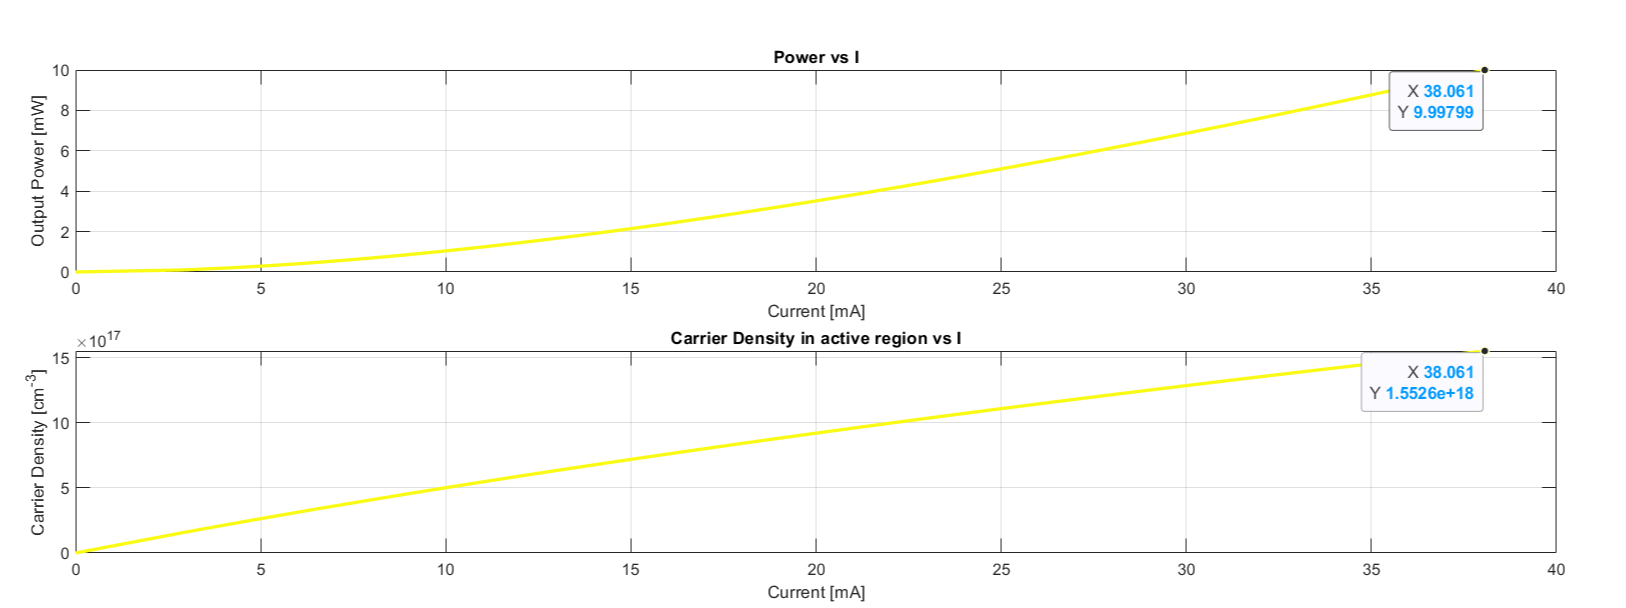
\includegraphics[width=15cm]{lab2/Images/prob1/P_N_vs_I_1.png}
  \caption{Andamento di $P_{out,opt}$ e di $N$ in funzione della corrente $I$ in ingresso al LED}
  \label{fig:P_N_vs_I_1}
\end{figure}

\noindent L'andamento della potenza ottica $P_{out,opt}$ osservabile nella Figura sopra riportata è in linea con il comportamento atteso tipico di un LED,
in quanto la potenza cresce linearmente con la corrente in ingresso al dispositivo. Per quanto riguarda la densità di portatori $N$, si nota un incremento monotono
all'aumentare della corrente, senza evidenziare fenomeni evidenti di saturazione nell'intervallo di valori considerato.

\subsection{Calcolo dell'efficienza radiativa $\boldsymbol{\eta_{rad}}$}
\noindent\\ Si può quindi procedere al calcolo dell'efficienza radiativa $\eta_{rad}$ del LED (\ref{eq:eta_rad}), definita come il rapporto tra il tasso di emissione spontanea $R_{sp}$
e il tasso di ricombinazione dei portatori $R_{rec}$:

\begin{equation}\label{eq:eta_rad}
    \eta_{rad} = \dfrac{R_{sp}}{R_{rec}} = \dfrac{R_{sp}}{R_{sp} + R_{nr}} =\dfrac{BN^2}{AN + BN^2 + CN^3}
\end{equation}
dove:
\begin{itemize}
    \item $R_{sp} = BN^2$ è il tasso di ricombinazione spontanea dei portatori (che in un materiale a gap diretto è radiativa);
    \item $R_{nr} = R_{nr,SRH} + R_{nr, Auger} = AN + CN^3$ è il tasso di ricombinazione non radiativa dei portatori;
    \item $R_{rec}$ è il tasso totale di ricombinazione dei portatori.
\end{itemize}

\noindent\\ Utilizzando il range di densità dei portatori $N$ estratto dalla simulazione precedente e i coefficienti ricombinativi del materiale ($A$, $B$ e $C$), è stato
calcolato l'andamento dell'efficienza radiativa $\eta_{\text{rad}}$, riportato in Figura \ref{fig:etar_vs_N_ext}. 

\noindent\\ Nell'intervallo di valori considerato, l'efficienza mostra un andamento monotono e quasi lineare. Tuttavia, ampliando il range della densità dei portatori a
valori superiori, si noterebbe che la curva raggiunge un valore massimo (pari a circa $\eta_{rad} \approx 0.53$, con $N \approx 10^{19}$ cm$^{-3}$) per poi iniziare a decrescere. Questo comportamento è legato alla "competizione"
tra i diversi meccanismi di ricombinazione: alle basse e medie densità il termine radiativo ($\propto BN^2$) cresce più rapidamente di quello SRH ($\propto AN$), rendendo
l'emissione spontanea dominante. Ad alte densità di portatori, al contrario, la ricombinazione non radiativa di tipo Auger ($\propto CN^3$) diventa preminente a causa della
dipendenza cubica da $N$, provocando la saturazione dell'efficienza e il suo successivo degrado.

\newpage

\begin{figure}[!h]
 \centering
 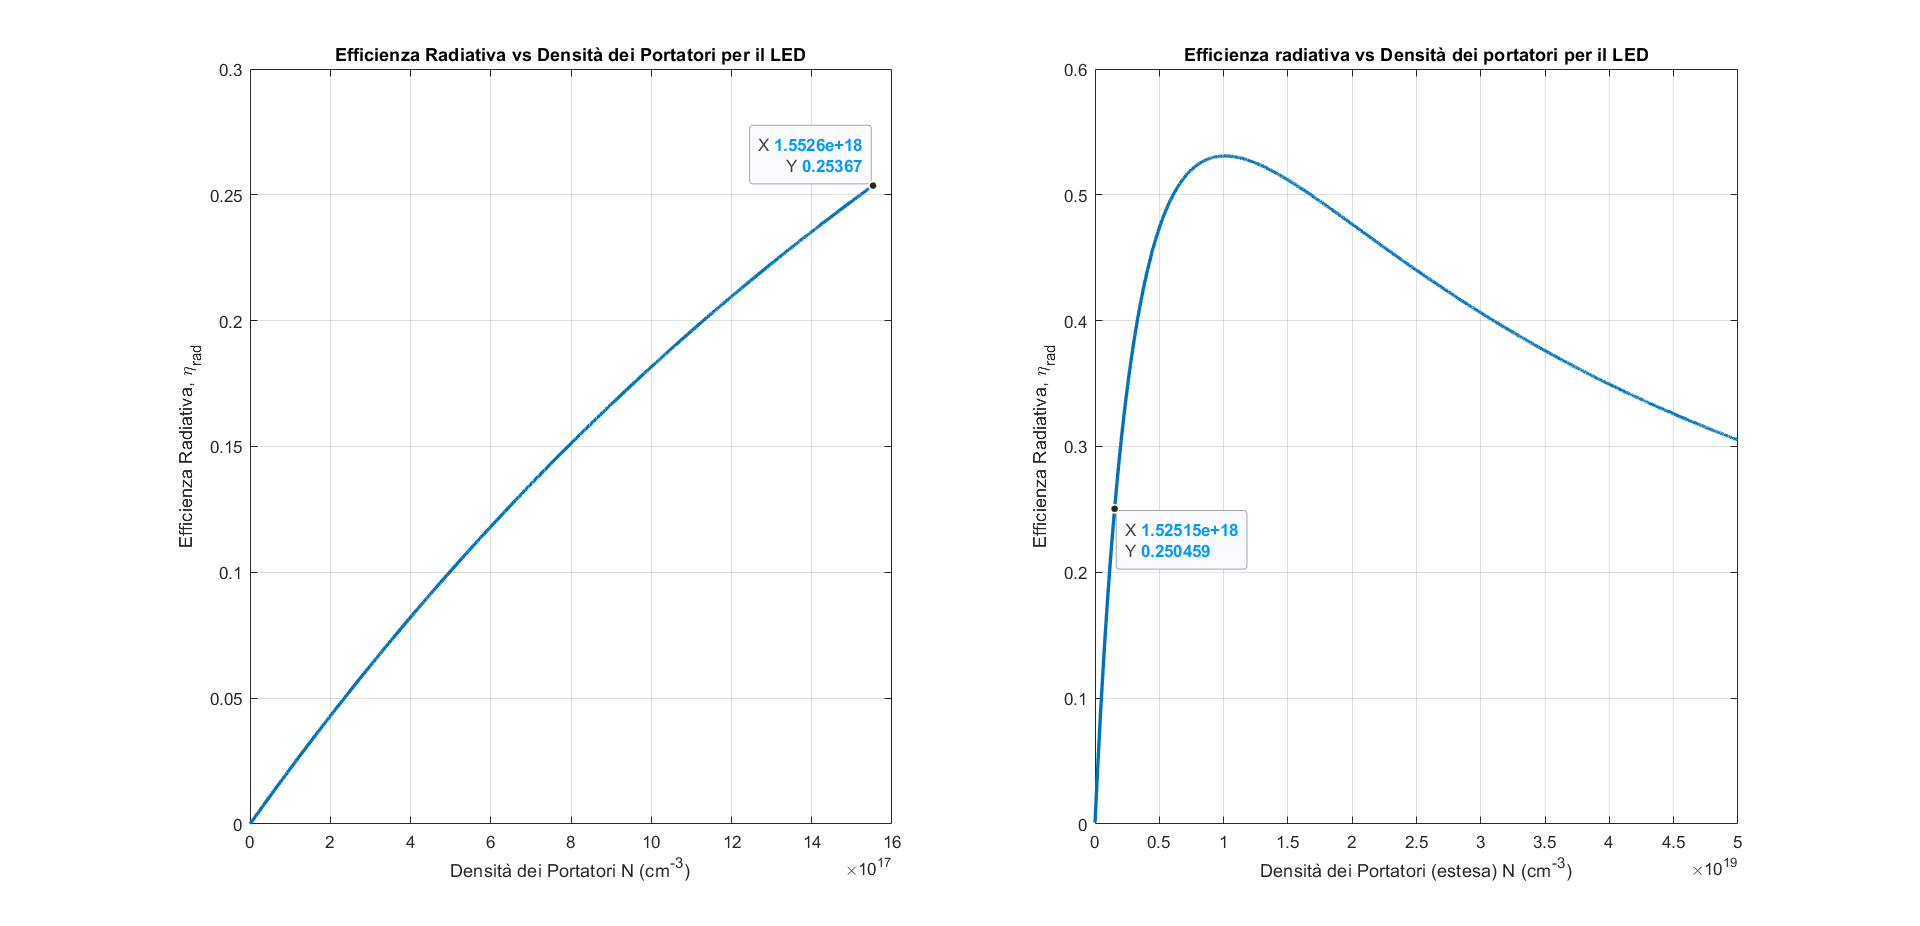
\includegraphics[width=15cm]{lab2/Images/prob1/etar_vs_N_ext.png}
  \caption{Andamento di $\eta_{\text{rad}}$ in funzione della densità dei portatori $N$.}
  \label{fig:etar_vs_N_ext}
\end{figure}

\subsection{Variazione dei parametri $A$, $B$ e $C$}
\noindent Variando opportunamente i coefficienti ricombinativi delle \textit{rate equations}, è possibile modulare il peso relativo dei diversi meccanismi di ricombinazione
all'interno della regione attiva. Imponendo come vincolo una variazione massima di un fattore $4$ rispetto ai valori nominali del materiale, sono stati analizzati due casi
limite:
\begin{itemize}
    \item \textbf{Caso 1 ($B = 4\times$, $A, C = 0.25\times$):} Massimizzazione dell'emissione spontanea e minimizzazione dei processi non radiativi ($R_{\text{sp}}$ massima e $R_{\text{nr}}$ minima).
    \item \textbf{Caso 2 ($B = 0.25\times$, $A, C = 4\times$):} Condizione opposta, caratterizzata da una forte soppressione dell'emissione spontanea in favore delle ricombinazioni non radiative ($R_{\text{sp}}$ minima e $R_{\text{nr}}$ massima).
\end{itemize}

\noindent Nelle Figure \ref{fig:P_N_vs_I_2} e \ref{fig:P_N_vs_I_3} sono riportati i grafici di $P_{\text{out}}$ e $N$ in funzione della corrente $I$ per i due casi limite sopra descritti.

\begin{figure}[!h]
    \centering
    \begin{subfigure}[b]{0.49\textwidth}
        \centering
        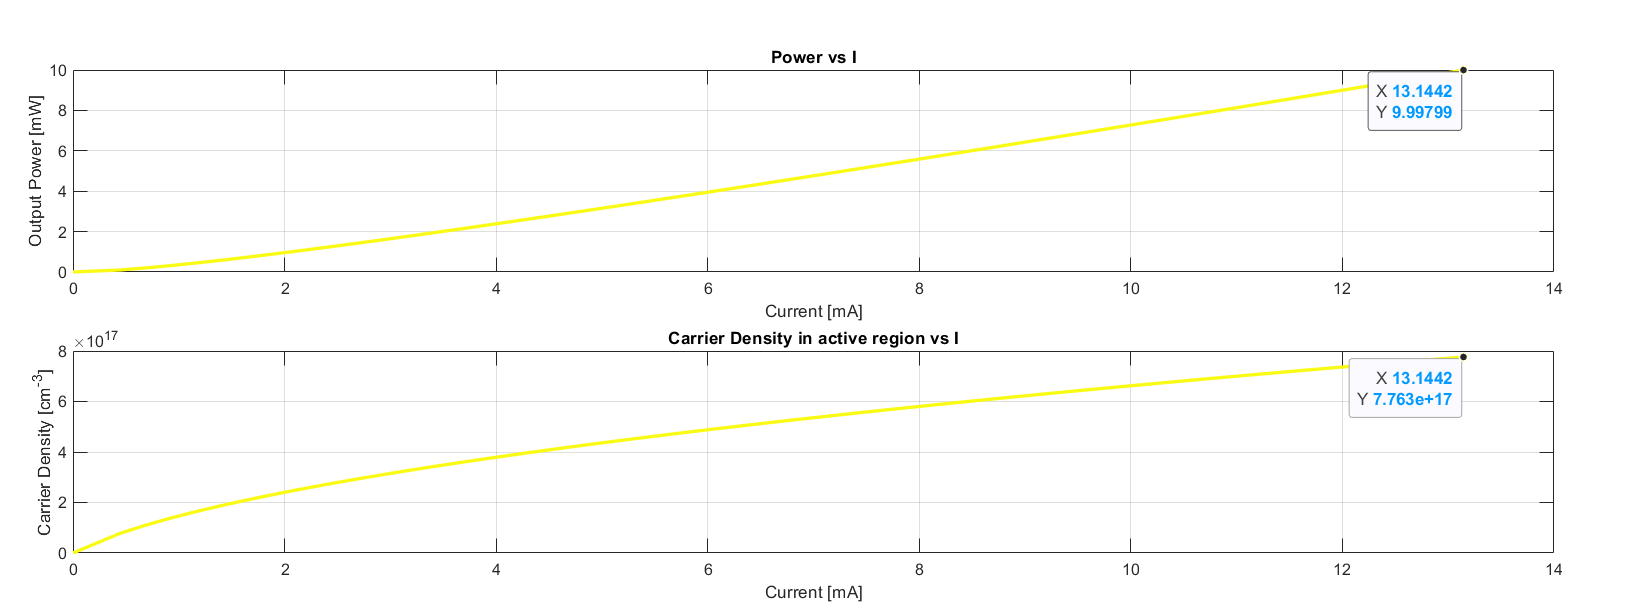
\includegraphics[width=\textwidth]{lab2/Images/prob1/P_N_vs_I_2.png}
        \caption{$P_{out,opt}$ e N vs I per il Caso 1}
        \label{fig:P_N_vs_I_2}
    \end{subfigure}
    \hfill
    \begin{subfigure}[b]{0.49\textwidth}
        \centering
        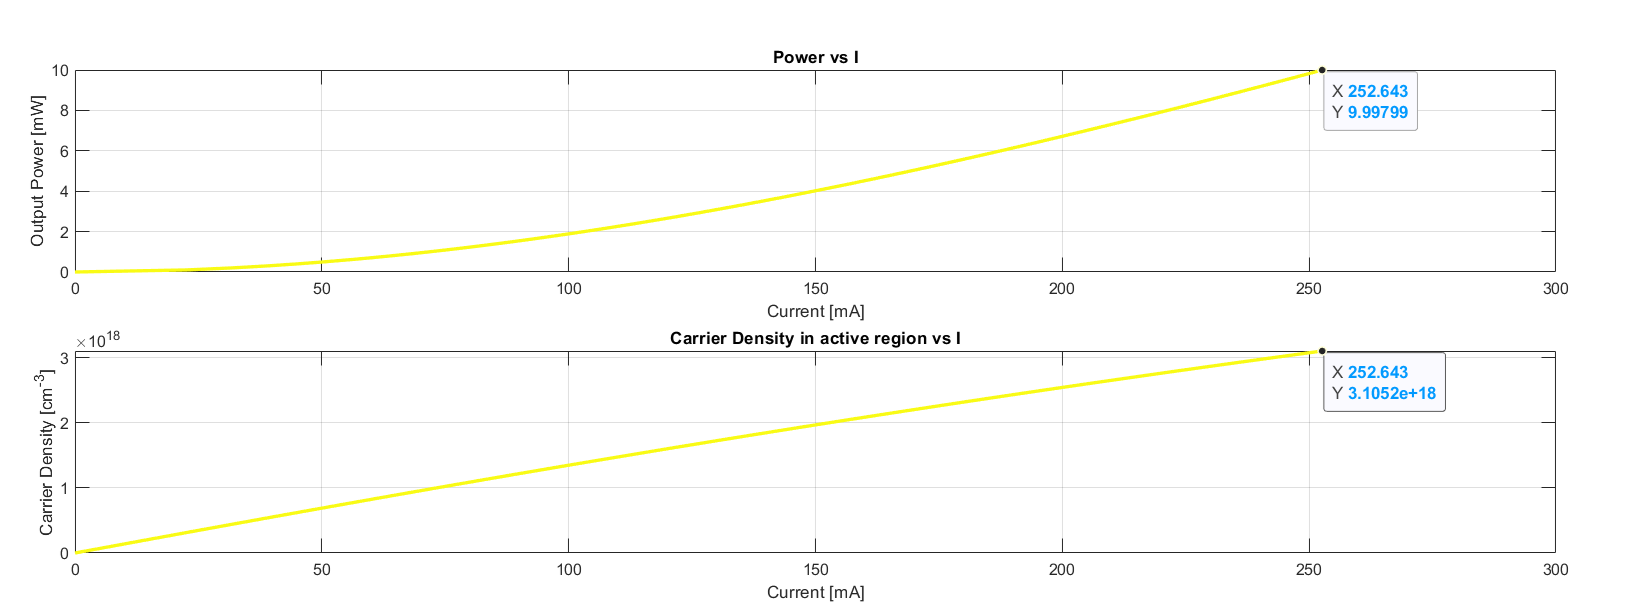
\includegraphics[width=\textwidth]{lab2/Images/prob1/P_N_vs_I_3.png}
        \caption{$P_{out,opt}$ e N vs I per il Caso 2}
        \label{fig:P_N_vs_I_3}
    \end{subfigure}
    \caption{$P_{out,opt}$ e di $N$ vs $I$ per i due casi limite di variazione dei coefficienti ricombinativi}
    \label{fig:P_N_vs_I_2_3}
\end{figure}

\noindent Dall'analisi dei grafici delle prestazioni $P_{\text{out}}$ e $N$ in funzione della corrente $I$ (Figura \ref{fig:P_N_vs_I_2_3}), si evidenziano differenze sostanziali nel
punto di funzionamento del dispositivo a parità di potenza ottica generata:
\begin{itemize}
    \item Nel \textbf{Caso 1}, per erogare la medesima potenza ottica del caso nominale, la corrente di alimentazione richiesta si riduce drasticamente a $13\text{ mA}$ (rispetto ai $38\text{ mA}$ del caso di \textit{default}). Parallelamente, anche la densità dei portatori accumulata nella regione attiva dimezza, passando da $1.552 \times 10^{18}\text{ cm}^{-3}$ a $7.763 \times 10^{17}\text{ cm}^{-3}$.
    \item Nel \textbf{Caso 2}, si osserva il comportamento opposto: per garantire la stessa $P_{\text{out}}$ è necessario erogare una corrente notevolmente più elevata, pari a circa $253\text{ mA}$, con una densità di portatori che sale fino a $3.1 \times 10^{18}\text{ cm}^{-3}$.
\end{itemize}

\noindent\\ Questa netta ripartizione dei tassi di ricombinazione si riflette direttamente sui valori di efficienza radiativa $\eta_{\text{rad}}$ ottenuti nei tre scenari, 
mostrati in Figura \ref{fig:etar_vs_N_all}.

\newpage

\begin{figure}[!h]
 \centering
 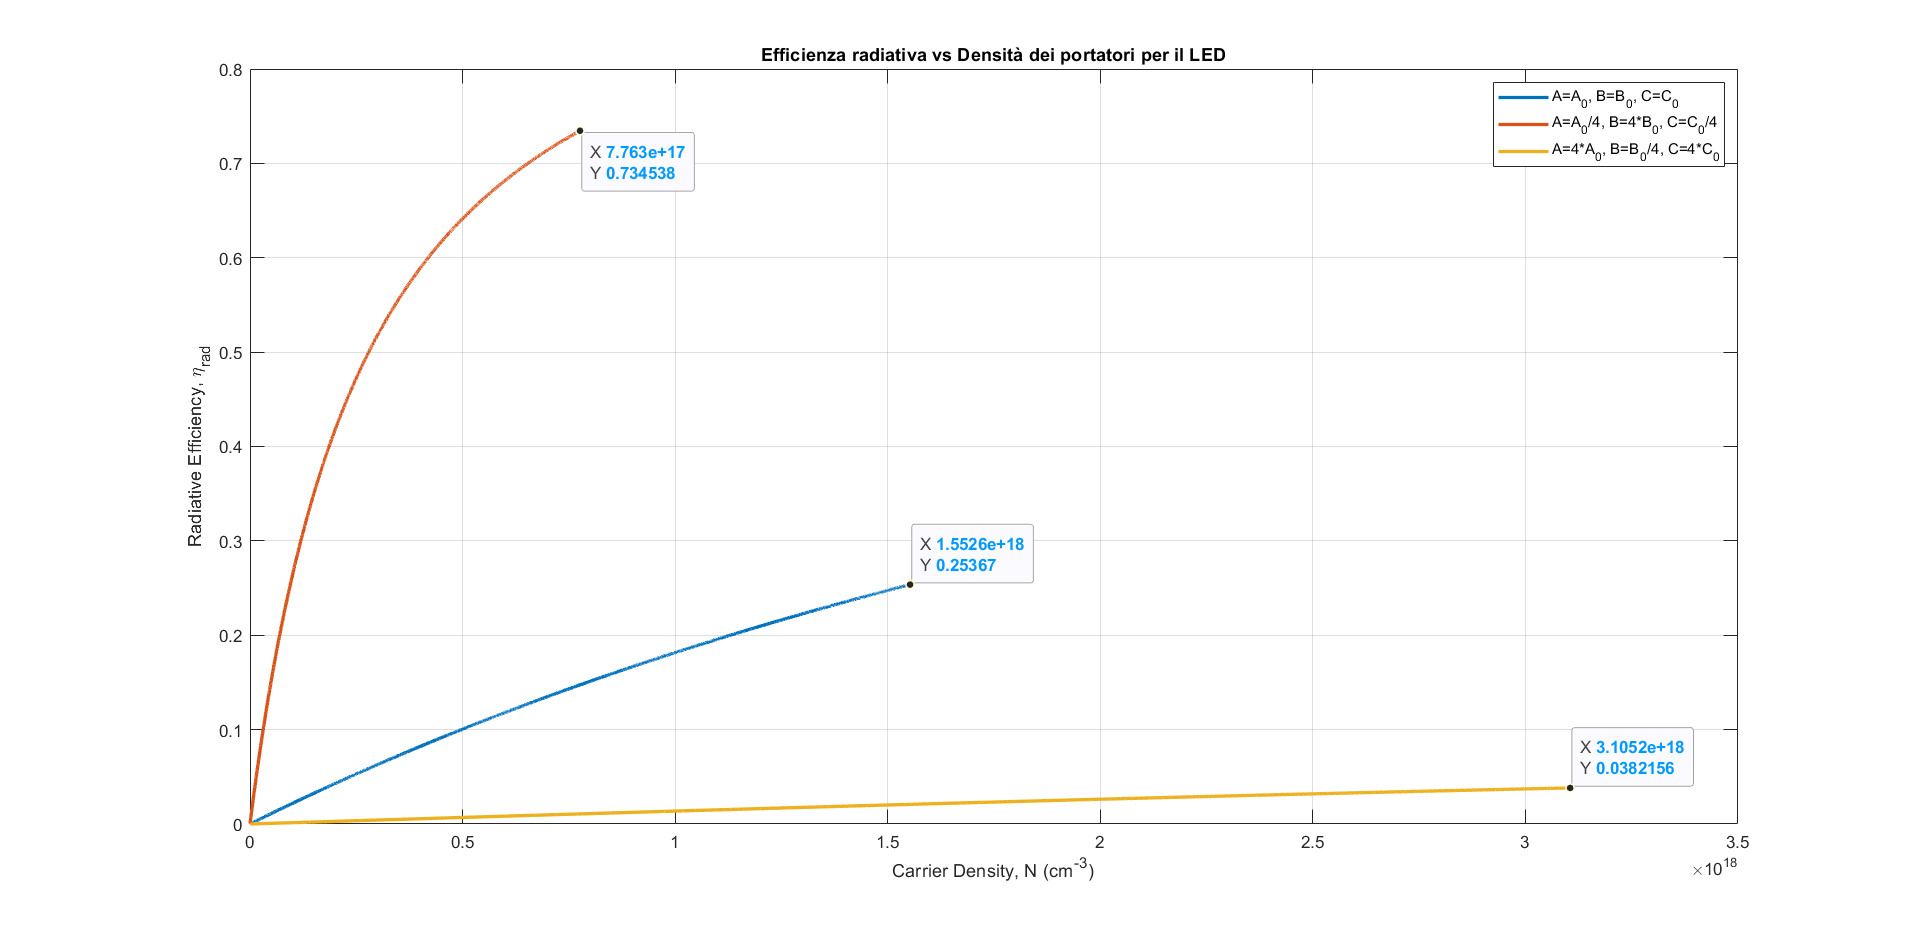
\includegraphics[width=15cm]{lab2/Images/prob1/etar_vs_N_all.png}
  \caption{Andamento di $\eta_{\text{rad}}$ vs $N$ nei 3 casi considerati: \textit{default}, Caso 1 e Caso 2}
  \label{fig:etar_vs_N_all}
\end{figure}

\noindent In particolare, è possibile riconoscere i seguenti comportamenti:
\begin{itemize}
    \item Nel caso di \textbf{\textit{default}}, l'efficienza raggiunge il valore massimo $\eta_{rad}\approx 0.254$ ($25.4\%$), con $N \approx 1.55 \times 10^{18}\text{ cm}^{-3}$ (mentre nel range esteso raggiungeva circa il $53\%$ con $N \approx 10^{19}\text{ cm}^{-3}$).
    \item Nel \textbf{Caso 1} ($B = 4\times$), la marcata dominanza dell'emissione spontanea porta l'efficienza radiativa a un valore massimo di circa il $73\%$ nell'intervallo di densità considerato ($N_{\text{max}} = 7.763 \times 10^{17}\text{ cm}^{-3}$).
    \item Nel \textbf{Caso 2} ($B = 0.25\times$), la forte incidenza delle perdite non radiative abbassa drásticamente l'efficienza $\eta_{\text{rad}}$, la quale raggiunge a stento il $3.8\%$ al valore massimo di densità dei portatori ($N_{\text{max}} = 3.1 \times 10^{18}\text{ cm}^{-3}$).
\end{itemize}
\noindent\\
\subsection{Transitorio di accensione}
\noindent Utilizzando la modalità \textit{Dynamic Analysis} del simulatore, è stato studiato il transitorio di accensione del LED, che corrisponde alla risposta del sistema
a un gradino di corrente in ingresso. Il segnale viene commutato a partire da un valore iniziale quasi nullo ($10^{-4} I/I_{\text{th}}$) fino a un valore a regime pari a
$6 I/I_{\text{th}} \approx 13.6 $ mA nell'intervallo temporale tra $3\text{ ns}$ e $30\text{ ns}$.

\noindent\\ L'andamento della densità di portatori $N(t)$ durante il transitorio di carica della regione attiva può essere descritto idealmente da una legge esponenziale
del primo ordine:
\begin{equation}
    N(t) = N(\infty) \left( 1 - e^{-\frac{t}{\tau}} \right)
\end{equation}
dove $N(\infty)$ rappresenta il valore della densità di portatori a regime permanente e $\tau$ è il tempo di vita dei portatori (\textit{carrier lifetime}). 

\noindent\\ Per stimare graficamente il valore di $\tau$ dal plot del transitorio, è sufficiente valutare la densità di portatori al tempo $t = \tau$:
\begin{equation}
    N(\tau) = N(\infty) \left( 1 - e^{-1} \right) \approx 0.632 \cdot N(\infty)
\end{equation}
Il tempo di vita dei portatori $\tau$ corrisponde quindi al tempo necessario affinché la densità di portatori raggiunga circa il $63.2\%$ del suo valore finale di
regime $N(\infty)$.

\newpage
\noindent\\\\ In Figura \ref{fig:P_N_vs_t1} è riportato il transitorio di accensione della potenza ottica in uscita $P_{\text{out}}$ e della densità di portatori
$N(t)$ per il caso con i parametri di \textit{default}. 

\begin{figure}[!h]
 \centering
 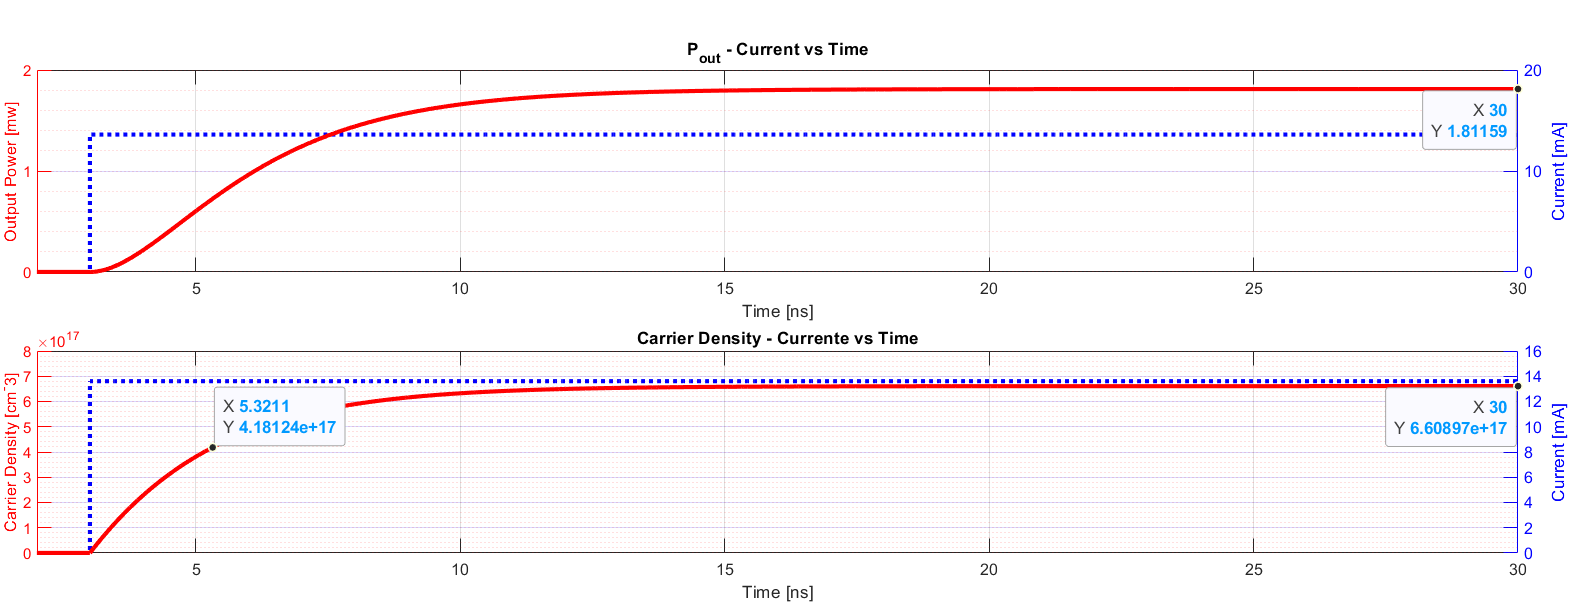
\includegraphics[width=15cm]{lab2/Images/prob1/P_N_vs_t1.png}
  \caption{Transitorio di accensione della potenza ottica $P_{\text{out}}$ e della densità dei portatori $N$ per il caso nominale (\textit{default}).}
  \label{fig:P_N_vs_t1}
\end{figure}

\noindent\\ Analogamente, l'analisi è stata ripetuta per i due casi limite di variazione dei parametri $A$, $B$ e $C$, ottenendo i transitori mostrati nelle Figure \ref{fig:P_N_vs_t2} e \ref{fig:P_N_vs_t3}.

\begin{figure}[!h]
 \centering
 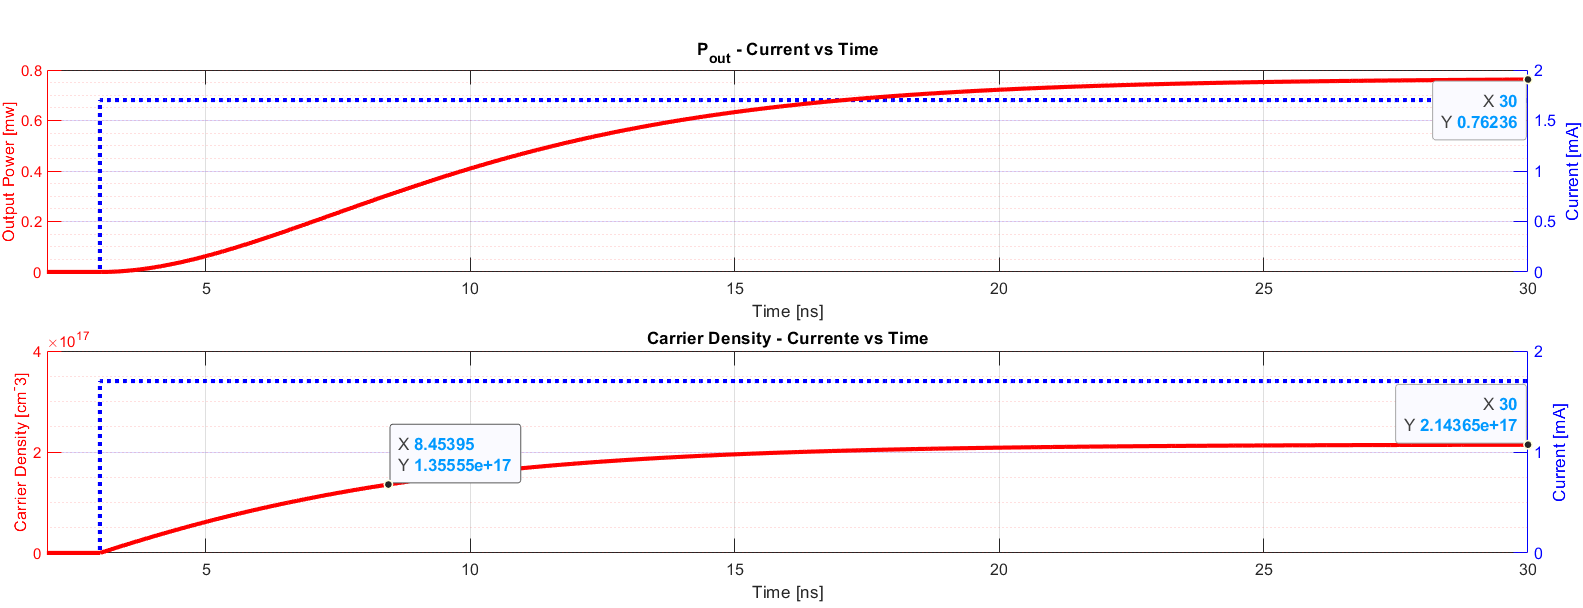
\includegraphics[width=15cm]{lab2/Images/prob1/P_N_vs_t2.png}
  \caption{Transitorio di accensione per il Caso 1 ($B = 4\times$, $A, C = 0.25\times$).}
  \label{fig:P_N_vs_t2}
\end{figure}

\begin{figure}[!h]
 \centering
 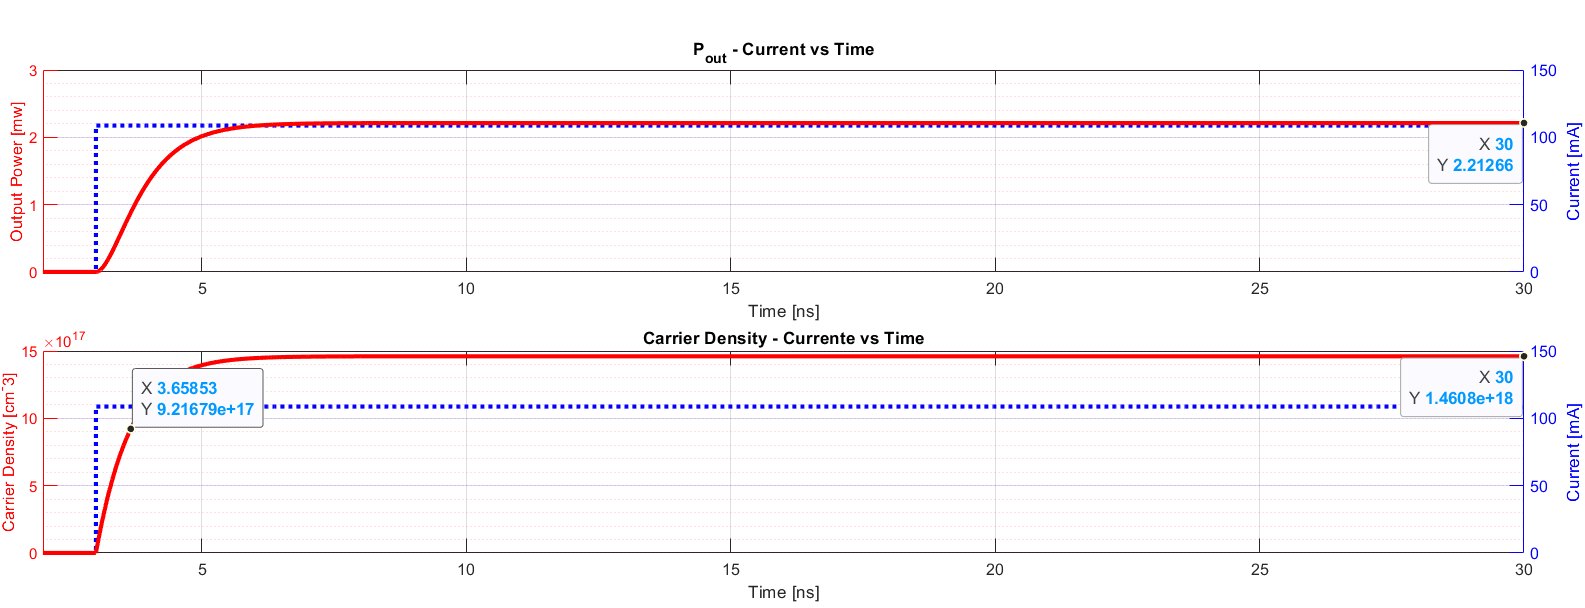
\includegraphics[width=15cm]{lab2/Images/prob1/P_N_vs_t3.png}
  \caption{Transitorio di accensione per il Caso 2 ($B = 0.25\times$, $A, C = 4\times$).}
  \label{fig:P_N_vs_t3}
\end{figure}

\newpage
\noindent Estraendo dai grafici i valori di $N(\infty)$ e applicando la condizione $N(\tau) = 0.632 \cdot N(\infty)$, sono stati stimati i tempi di vita dei portatori per i tre scenari considerati, i quali sono riassunti in Tabella \ref{tab:carrier_lifetime}.

\begin{table}[!h]
\centering
\begin{tabular}{|l|c|c|c|}
\hline
\textbf{Caso} & $N(\infty)$ [\text{cm}$^{-3}$] & $N(\tau)$ [\text{cm}$^{-3}$] & $\tau$ [\text{ns}] \\ \hline\hline
\textbf{Default} & $6.609 \times 10^{17}$ & $4.178 \times 10^{17}$ & 2.32 \\ \hline
\textbf{Caso 1} ($B = 4\times$) & $2.144 \times 10^{17}$ & $1.355 \times 10^{17}$ & 5.45 \\ \hline
\textbf{Caso 2} ($B = 0.25\times$) & $1.461 \times 10^{18}$ & $9.235 \times 10^{17}$ & 0.66 \\ \hline
\end{tabular}
\caption{Valori del tempo di vita dei portatori $\tau$ al variare dei parametri di ricombinazione}
\label{tab:carrier_lifetime}
\end{table}

\noindent Come si evince dai dati, la variazione dei coefficienti $A$, $B$ e $C$ modifica significativamente il tempo di vita dei portatori $\tau$. Ricordando la relazione
che lega il tasso di ricombinazione totale al tempo di vita medio dei portatori:
\begin{equation}
R_{\text{rec}} = AN + BN^2 + CN^3 \approx \frac{N}{\tau} \implies \frac{1}{\tau} \approx A + BN + CN^2
\end{equation}

\noindent Nel \textbf{Caso 1}, la drastica riduzione del coefficiente di ricombinazione SRH ($A = 0.25\times$) e il minore accumulo di portatori a regime $N(\infty)$
riducono la somma dei termini $A + BN + CN^2$. Di conseguenza, $1/\tau$ diminuisce e si ottiene un incremento del tempo di vita dei portatori $\tau$, prolungando il
transitorio di carica della regione attiva. 

\noindent\\ Al contrario, nel \textbf{Caso 2}, l'incremento dei coefficienti non radiativi ($A, C = 4\times$) unitamente all'elevata densità di portatori $N(\infty)$
necessaria a regime aumenta notevolmente la frequenza delle ricombinazioni, riducendo nettamente il valore di $\tau$ e velocizzando la risposta temporale.

%%%%%%%%%%%%%%% PROBLEMA 2 %%%%%%%%%%%%%%%%%%%%%%%%

\newpage
\section{Analisi di piccolo segnale del LED}
\noindent Per valutare la dinamica di piccolo segnale del LED, è stata impiegata la modalità \textit{Dynamic Analysis}, applicando un piccolo gradino di corrente sovrapposto
a un valore di polarizzazione (\textit{bias}). Per garantire che il dispositivo raggiunga lo stato stazionario prima dell'applicazione della perturbazione, il valore di
\textit{Step Start Time} è stato impostato a $30\text{ ns}$, mentre lo \textit{Step End Time} è stato fissato a $60\text{ ns}$, intervallo sufficientemente lungo da
assicurare che sia la potenza $P_{{out,opt}}(t)$ che i portatori $N(t)$ raggiungano il loro valore limite, quindi il regime stazionario.

\noindent\\ In Figura \ref{fig:P_N_vs_t_b1_1} è riportata la risposta temporale della densità di portatori $N(t)$ e della potenza ottica $P_{\text{out}}(t)$ a un
bias $I_b = 6 I_{\text{th}}$, dove si evidenzia il raggiungimento del regime stazionario prima dell'istante di commutazione e dopo la perturbazione.

\begin{figure}[!h]
 \centering
 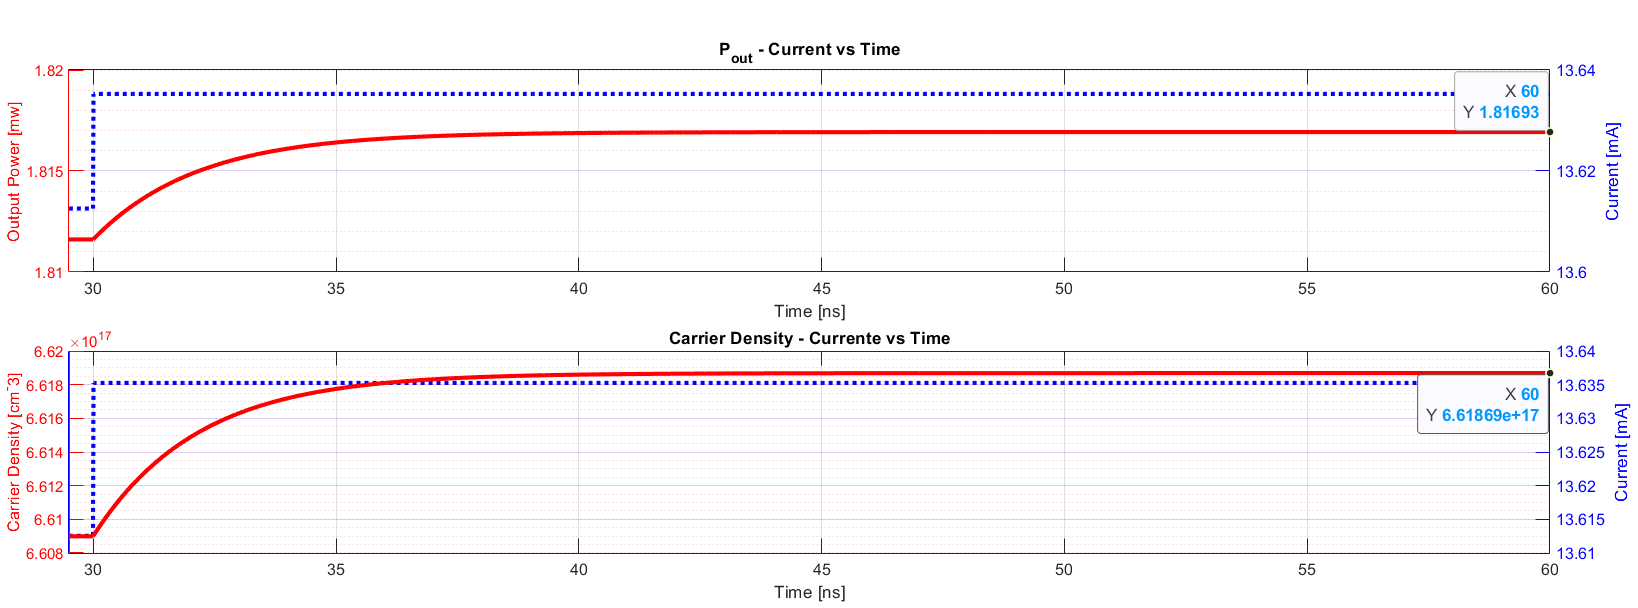
\includegraphics[width=14cm]{lab2/Images/prob2/P_N_vs_t_b1_1.png}
  \caption{Risposta temporale al piccolo gradino di corrente con $I_b = 6 I_{\text{th}}$, $t_{\text{start}} = 30\text{ ns}$ e $t_{\text{end}} = 60\text{ ns}$.}
  \label{fig:P_N_vs_t_b1_1}
\end{figure}

\noindent\\ Tramite l'operazione di calcolo della risposta di modulazione di ampiezza (\textit{Calculate AM}), si è ottenuta la risposta in frequenza della potenza ottica
modulata. L'analisi è stata prima condotta variando la corrente di polarizzazione $I_b$ sui valori $6 I_{\text{th}}$, $3 I_{\text{th}}$ e $1 I_{\text{th}}$ mantenendo i
parametri $A$, $B$ e $C$ al valore di \textit{default}. I risultati ottenuti sono riportati nelle Figure \ref{fig:AM_b1_1} e \ref{fig:AM_b2_b3}.

\begin{figure}[!h]
 \centering
 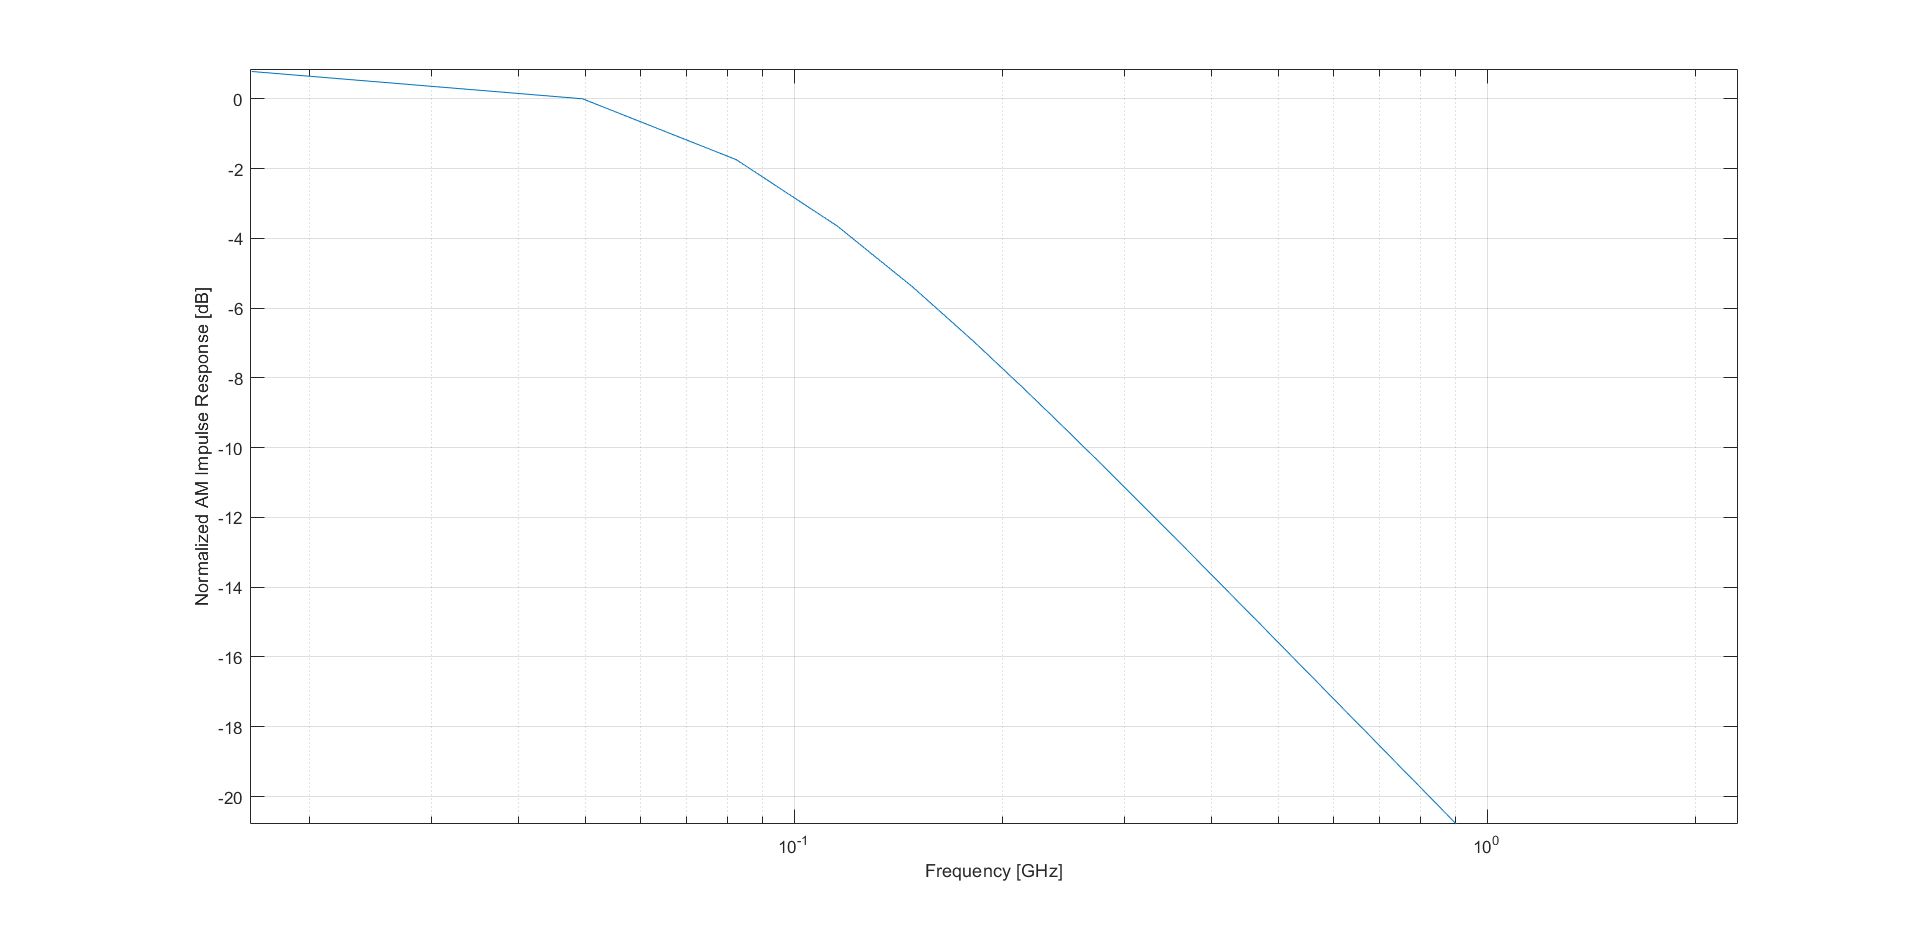
\includegraphics[width=15cm]{lab2/Images/prob2/AM_b1_1.png}
  \caption{Risposta di modulazione AM del LED con corrente di polarizzazione $I_b = 6 I_{\text{th}}$}
  \label{fig:AM_b1_1}
\end{figure}

\newpage
\begin{figure}[!h]
    \centering
    \begin{subfigure}[b]{0.49\textwidth}
        \centering
        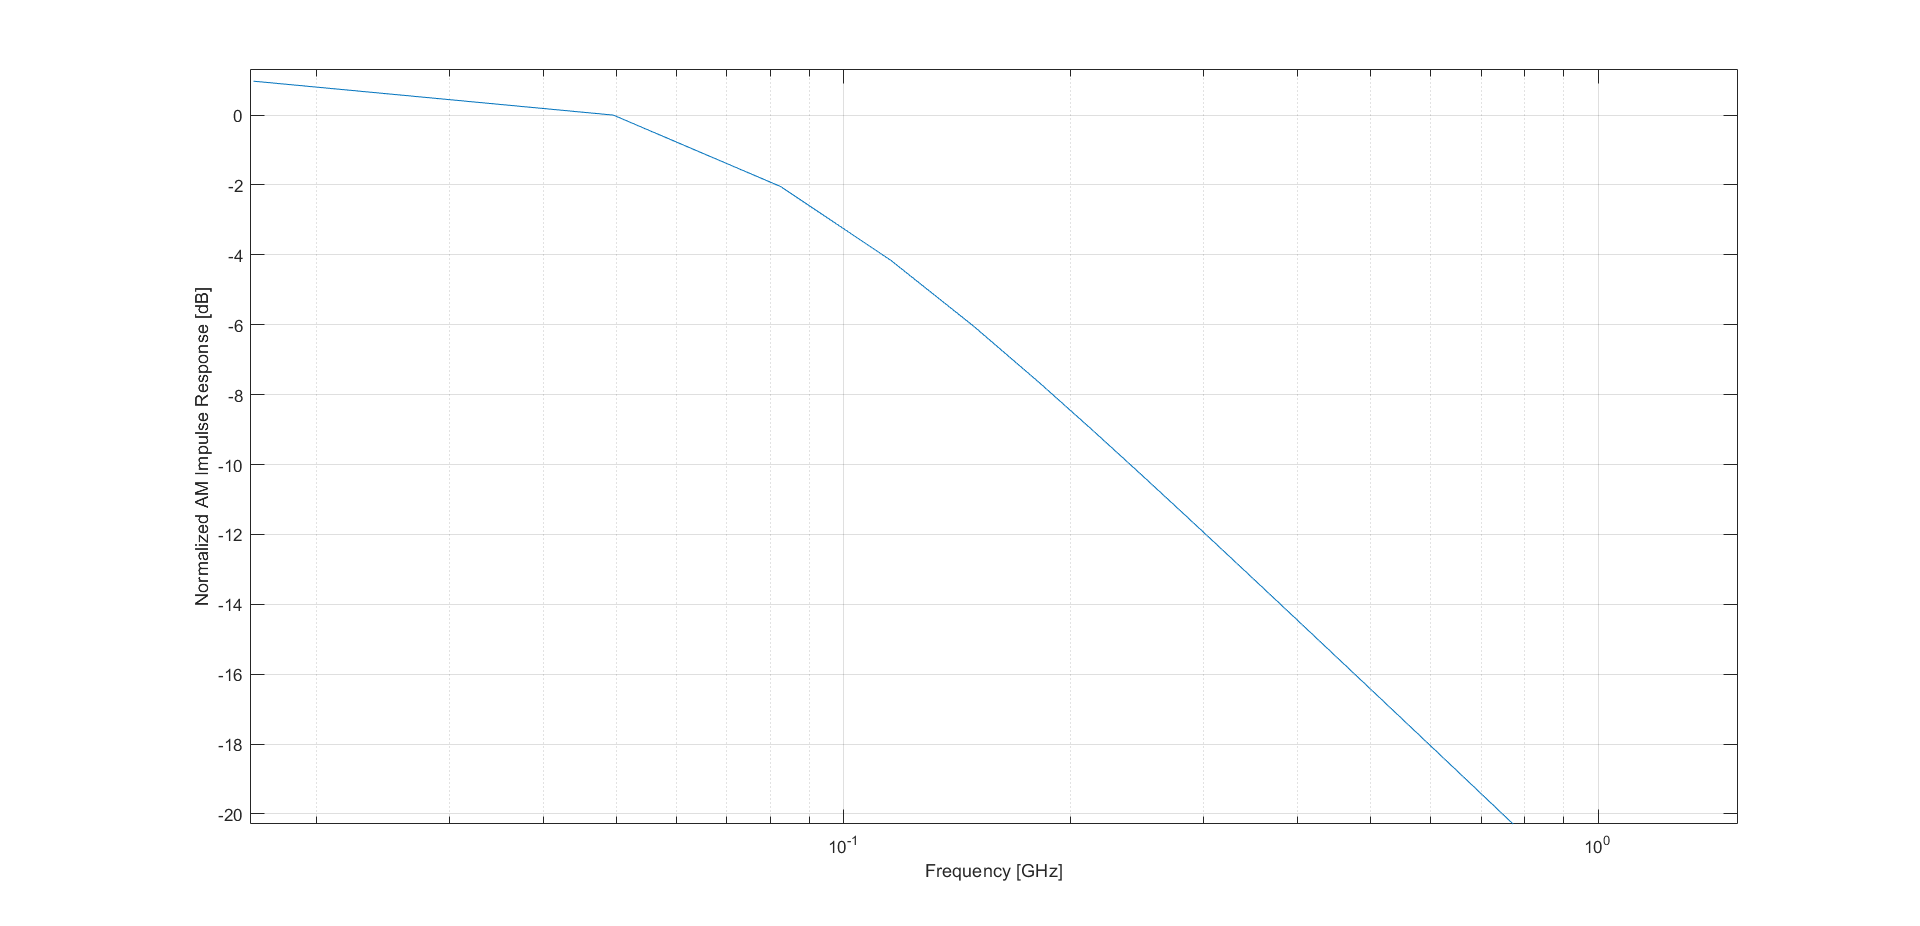
\includegraphics[width=\textwidth]{lab2/Images/prob2/AM_b2_1.png}
        \caption{Risposta AM del LED con $I_b = 3 I_{\text{th}}$}
        \label{fig:AM_b2_1}
    \end{subfigure}
    \hfill
    \begin{subfigure}[b]{0.49\textwidth}
        \centering
        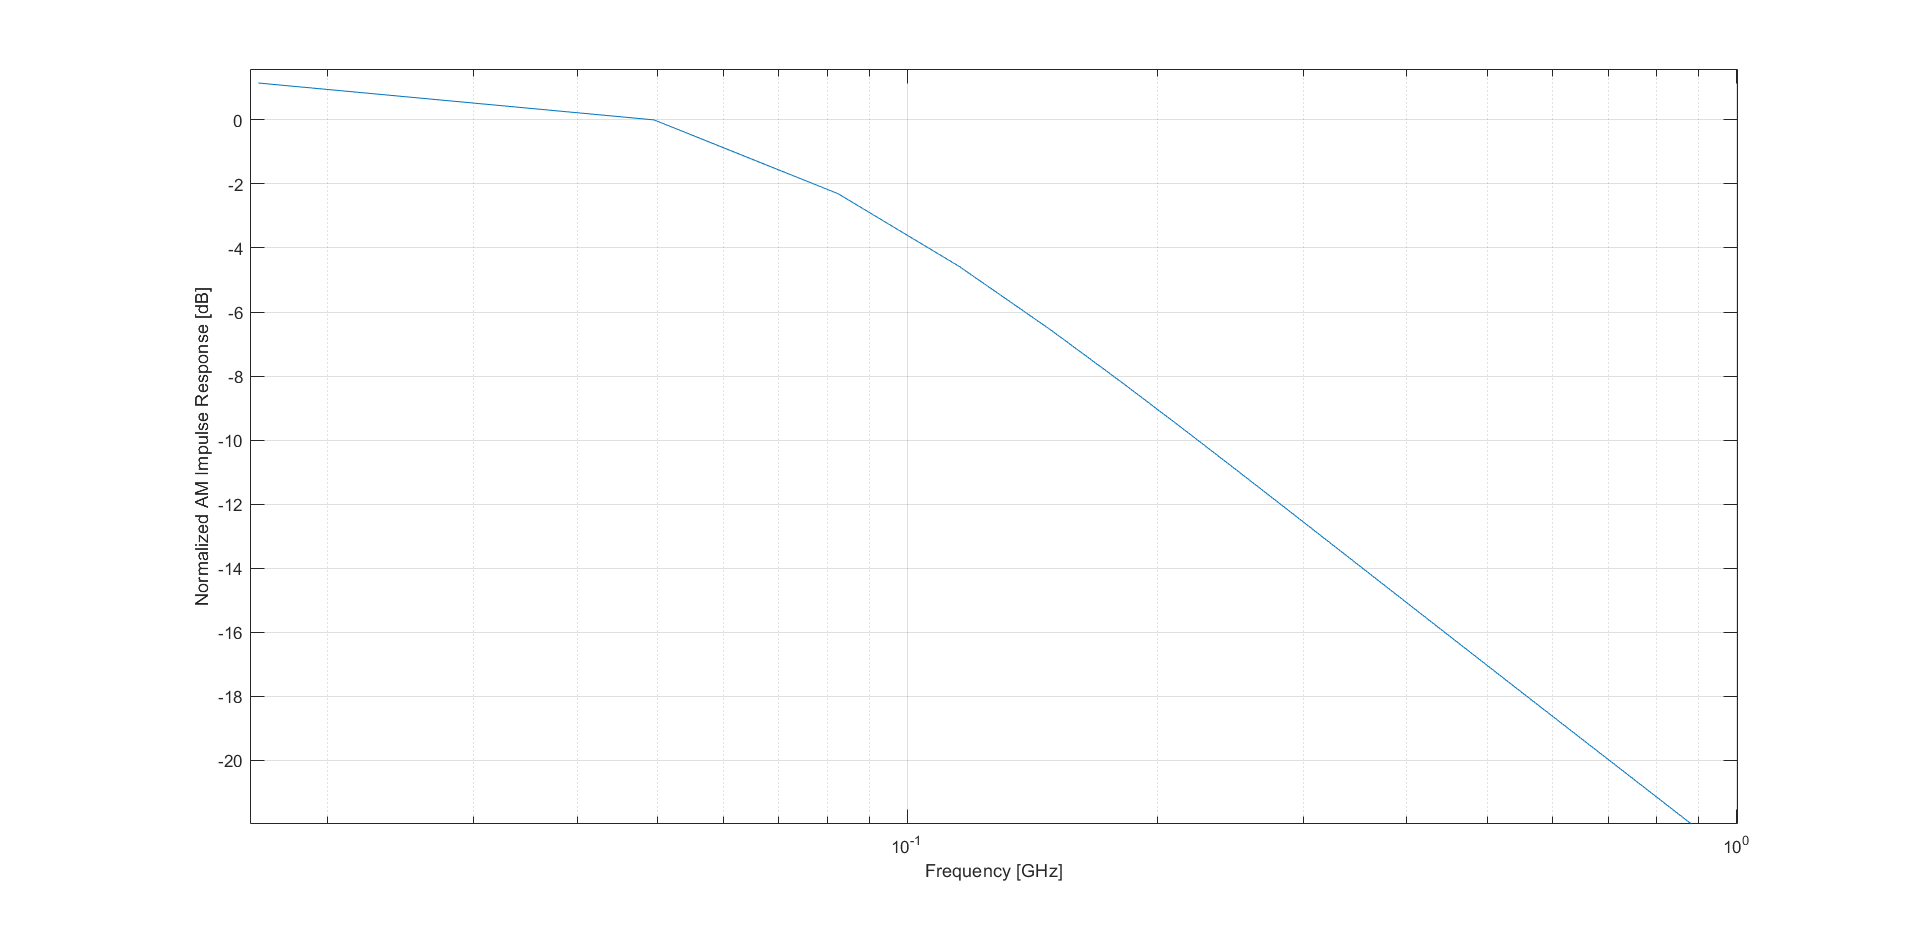
\includegraphics[width=\textwidth]{lab2/Images/prob2/AM_b3_1.png}
        \caption{Risposta AM del LED con $I_b = 1 I_{\text{th}}$}
        \label{fig:AM_b3_1}
    \end{subfigure}
    \caption{Risposta AM del LED con correnti di polarizzazione $I_b = 3 I_{\text{th}}$ e $I_b = 1 I_{\text{th}}$}
    \label{fig:AM_b2_b3}
\end{figure}

\noindent Successivamente, fissando la corrente al livello di bias $I_b = 6 I_{\text{th}}$, sono state valutate le
risposte in frequenza nei due casi limite di variazione dei coefficienti $A$, $B$ e $C$.\\ I grafici ottenuti nel \textbf{Caso 1} e nel \textbf{Caso 2} sono riportati
in Figura \ref{fig:AM_b1_2} e \ref{fig:AM_b1_3} rispettivamente.

\begin{figure}[!h]
 \centering
 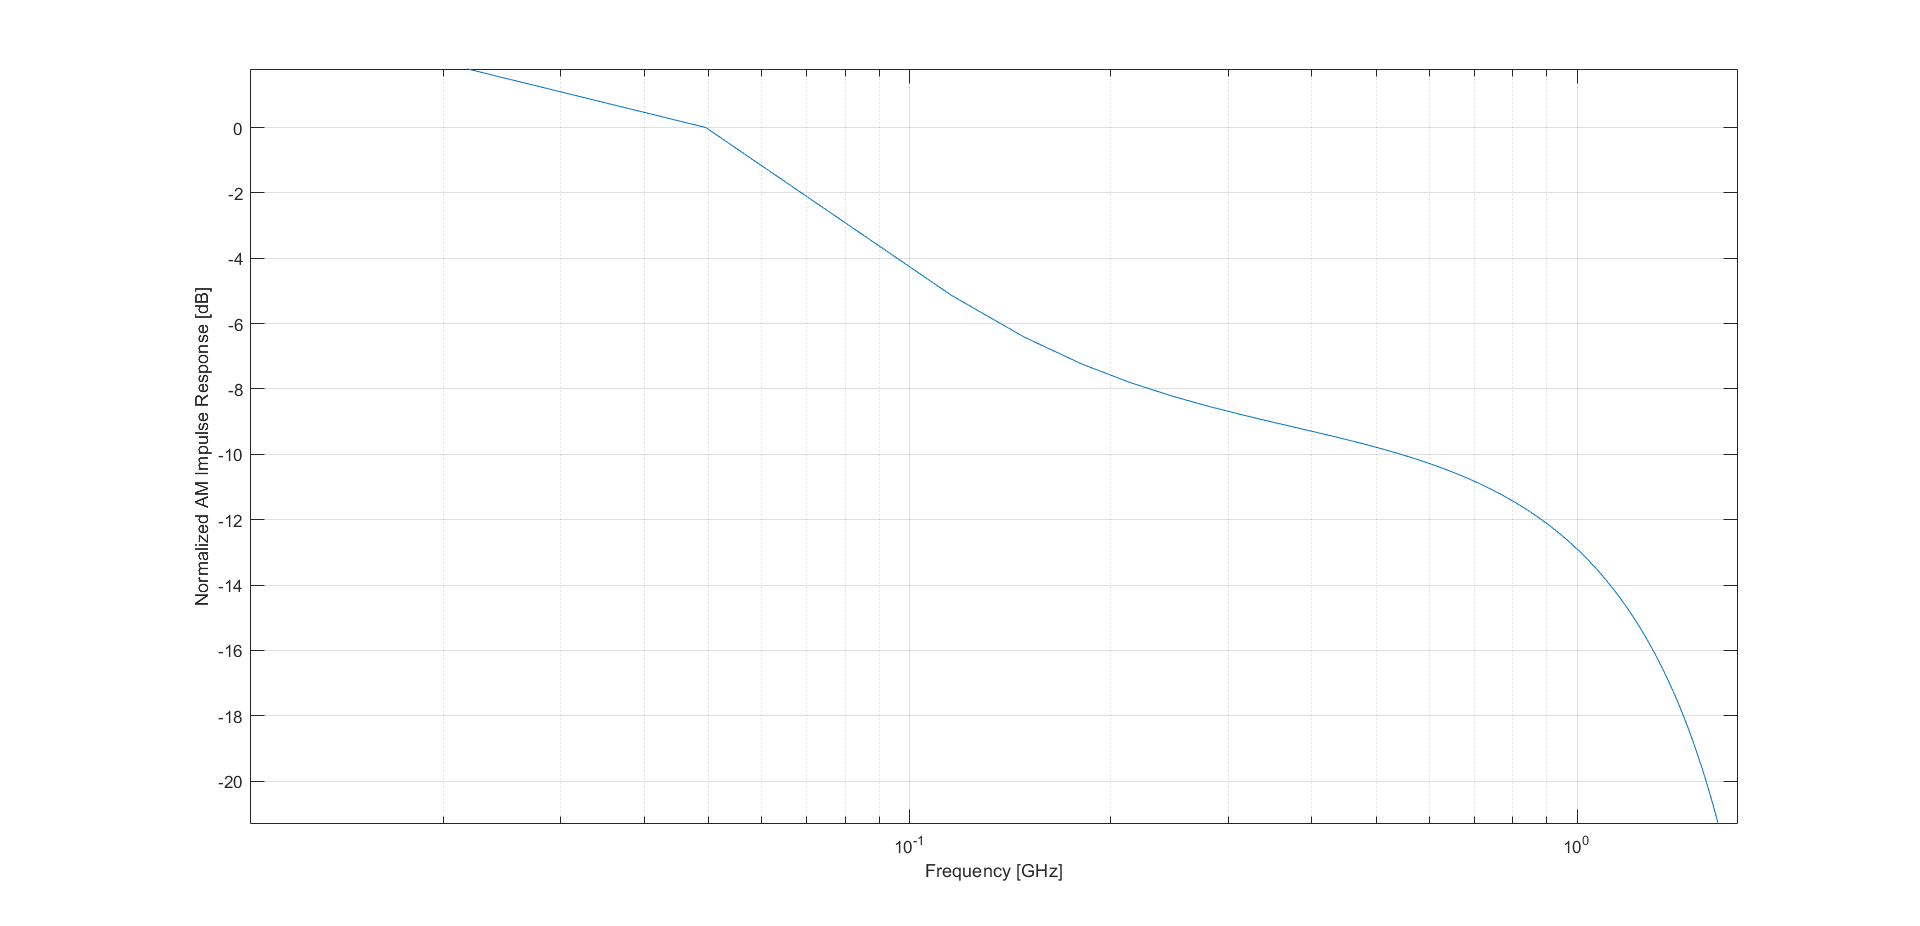
\includegraphics[width=15cm]{lab2/Images/prob2/AM_b1_2.png}
  \caption{Risposta di modulazione AM a $I_b = 6 I_{\text{th}}$ - Caso 1 ($B = 4\times$)}
  \label{fig:AM_b1_2}
\end{figure}

\begin{figure}[!h]
 \centering
 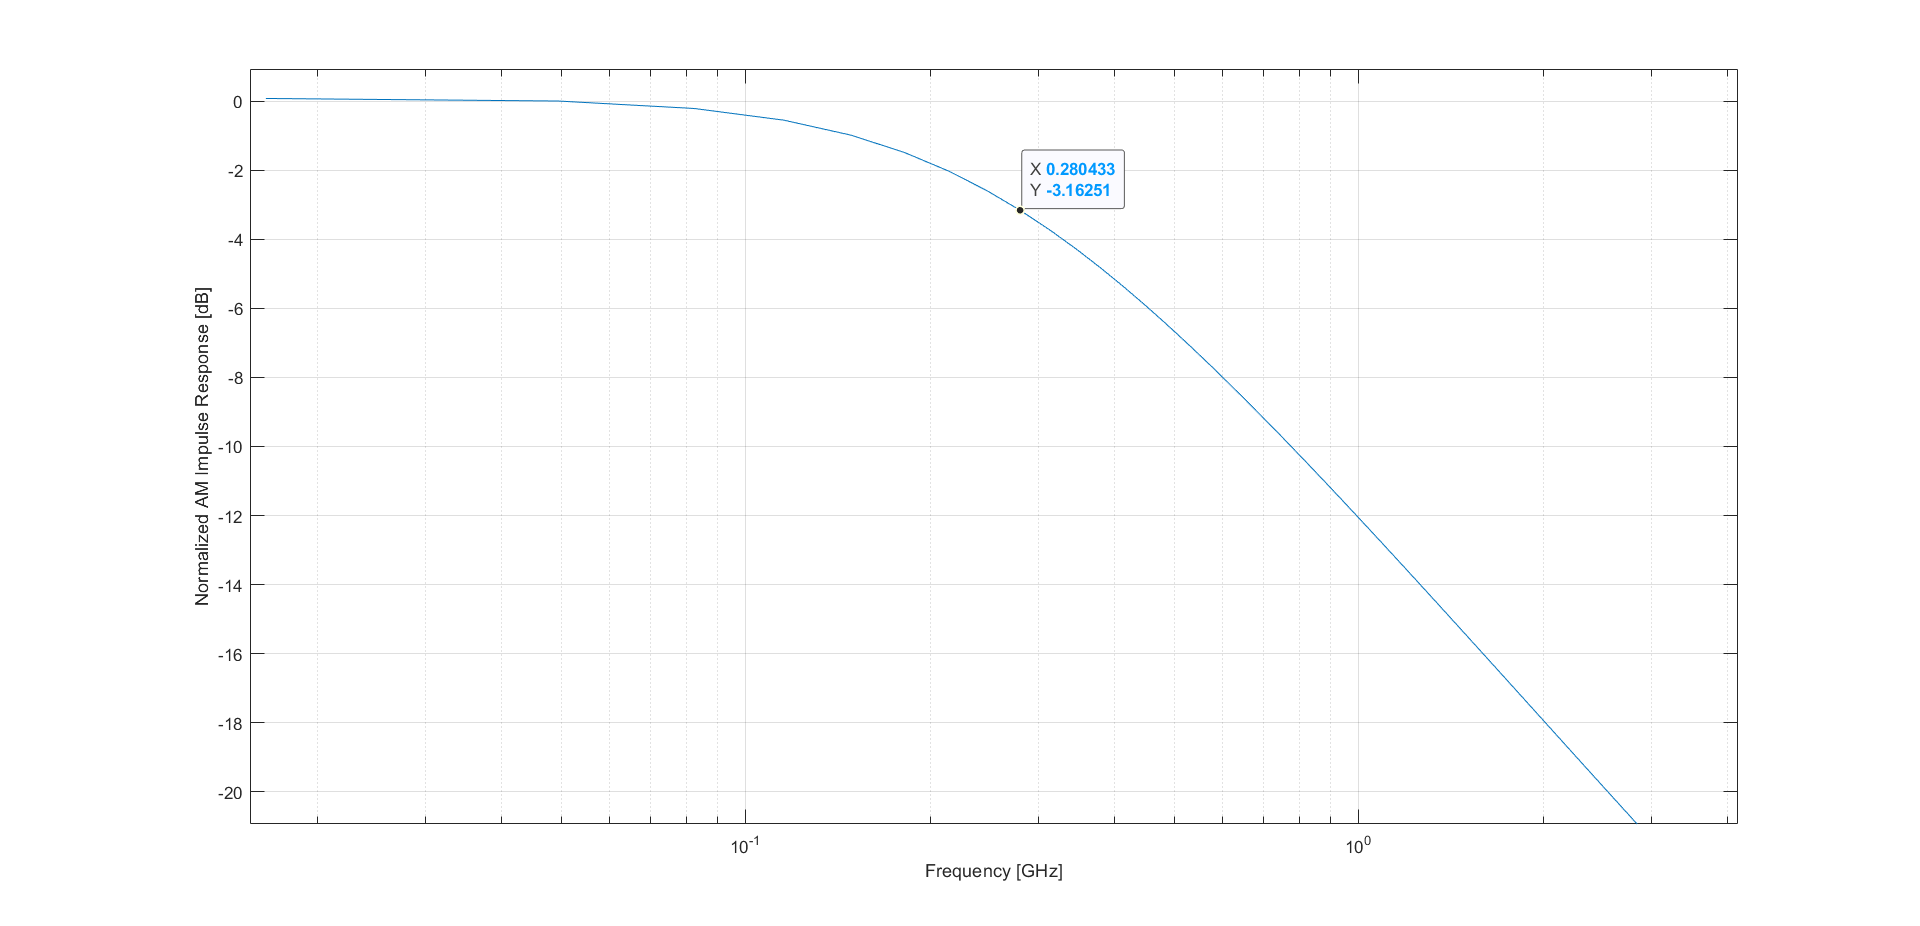
\includegraphics[width=15cm]{lab2/Images/prob2/AM_b1_3.png}
  \caption{Risposta di modulazione AM a $I_b = 6 I_{\text{th}}$ - Caso 2 ($B = 0.25\times$)}
  \label{fig:AM_b1_3}
\end{figure}

\newpage
\noindent Dai grafici delle risposte AM sono state misurate le larghezze di banda a $-3\text{ dB}$ ($f_{-3\text{dB}}$). I risultati ottenuti sono sintetizzati
nella Tabella \ref{tab:bandwidth_summary}.

\begin{table}[!h]
\centering
\begin{tabular}{|l|c|c|}
\hline
\textbf{Configurazione A, B, C} & \textbf{Corrente di Bias $\boldsymbol{{I_b}}$} & $\boldsymbol{f_{-3dB}}$ \textbf{[MHz]} \\ \hline\hline
\textbf{Default} & $1 I_{\text{th}}$ & 90 \\ \hline
\textbf{Default} & $3 I_{\text{th}}$ & 95 \\ \hline
\textbf{Default (Riferimento)} & $\boldsymbol{6 I_{th}}$ & $\boldsymbol{100}$ \\ \hline\hline
\textbf{Caso 1} ($B = 4\times$) & $6 I_{\text{th}}$ & 80 \\ \hline
\textbf{Caso 2} ($B = 0.25\times$) & $6 I_{\text{th}}$ & 280 \\ \hline
\end{tabular}
\caption{Larghezze di banda di modulazione a $-3\text{ dB}$ per le diverse correnti di bias e configurazioni dei parametri ricombinativi.}
\label{tab:bandwidth_summary}
\end{table}

\noindent La funzione di trasferimento di piccolo segnale di un LED presenta un comportamento simile a quello di un
filtro passa-basso del primo ordine del tipo:
\begin{equation}
H(\omega) = \frac{1}{j\omega + \frac{1}{\tau}} \implies f_{-3dB} = \frac{1}{2\pi \tau}
\end{equation}
Ne consegue che la frequenza di taglio a $-3\text{ dB}$ è inversamente proporzionale al tempo di vita dei portatori $\tau$. Inoltre, dato il legame tra $\tau$ e la densità
di portatori $N$:
\begin{equation}
    \frac{N}{\tau} \approx R_{rec} = AN + BN^2 + CN^3 \implies \frac{1}{\tau} \approx A + BN + CN^2
\end{equation}

\noindent è possibile esprimere la banda a $-3\text{ dB}$ in funzione del numero di portatori $N$ come segue:
\begin{equation}
f_{-3\text{dB}} = \frac{1}{2\pi \tau} \approx \frac{1}{2\pi} \left( A + 2BN + 3CN^2 \right)
\end{equation}

\noindent\\ I dati mostrano chiaramente due tendenze fisiche fondamentali:
\begin{enumerate}
    \item \textbf{Dipendenza dal bias:} Aumentando la corrente $I_b$ da $1 I_{\text{th}}$ a $6 I_{\text{th}}$, la densità di portatori a regime $N$ cresce. Di conseguenza,
    i termini ricombinativi $\propto BN$ e $\propto CN^2$ aumentano, riducendo $\tau$ e incrementando la banda di modulazione $f_{-3\text{dB}}$.
    \item \textbf{Dipendenza da $A, B, C$:} Nel \textbf{Caso 1}, il valore di $\tau$ più elevato (riscontrato nell'analisi transitoria a causa del ridotto valore di $A$ e
    della minore densità $N$) determina una banda di modulazione $f_{-3\text{dB}}$ più stretta. Viceversa, nel \textbf{Caso 2}, l'elevata frequenza di ricombinazione non
    radiativa riduce $\tau$, traducendosi in una larghezza di banda nettamente maggiore ($\approx 280$ MHz) a scapito dell'efficienza radiativa.
\end{enumerate}

\subsubsection{Relazione tra Banda di Modulazione ed Efficienza Radiativa:}
Risulta evidente l'esistenza di un \textit{trade-off} intrinseco tra la risposta in frequenza e l'efficienza di un LED. Ricordando che:
\[
\eta_{\text{rad}} \approx \frac{BN^2}{AN + BN^2 + CN^3} \quad,\quad f_{-3\text{dB}} \approx \frac{1}{2\pi}\frac{R_{\text{rec}}}{N} = \frac{1}{2\pi} \left( A + BN + CN^2 \right)
\]

\noindent si nota che un aumento delle ricombinazioni non radiative ($A$ o $C$) riduce $\eta_{\text{rad}}$ ma
aumenta la velocità del dispositivo (e quindi $f_{-3\text{dB}}$). Massimizzare l'efficienza radiativa comporta inevitabilmente un prolungamento del tempo di vita dei portatori
$\tau$, limitando la massima velocità di modulazione del LED.

%%%%%%%%%%%%%%%%% PROBLEMA 3 %%%%%%%%%%%%%%%%%%%%%%

\newpage
\section{PRBS: modulazione ad ampio segnale del LED}
\noindent Per valutare le prestazioni del LED con una modulazione di ampio segnale, è stata utilizzata la modalità \textit{PRBS Analysis} all'interno del tool
\textit{Dynamic Analysis}.\\ Il dispositivo è stato sottoposto a una sequenza binaria pseudo-casuale (\textit{Pseudo Random Bit Sequence}) commutando la corrente tra un
livello minimo $I_{\text{min}} = 0.1 I_{\text{th}}$ (stato logico $'0'$) e un livello massimo $I_{\text{max}} = 6 I_{\text{th}}$ (stato logico $'1'$).

\noindent\\ Poiché la durata del singolo bit è inversamente proporzionale al bit-rate ($T_b = 1/B_r$), la velocità di variazione del segnale d'ingresso determina
la capacità della potenza ottica $P_{\text{out}}(t)$ e della densità di portatori $N(t)$ di "inseguire" il profilo la corrente. Nelle Figure \ref{fig:10M},
\ref{fig:100M}, \ref{fig:1G} e \ref{fig:2_5G} sono mostrati gli andamenti temporali di $P_{\text{out}}$ e $N$ a diversi bit-rate ($B_r$).

\begin{figure}[!h]
 \centering
 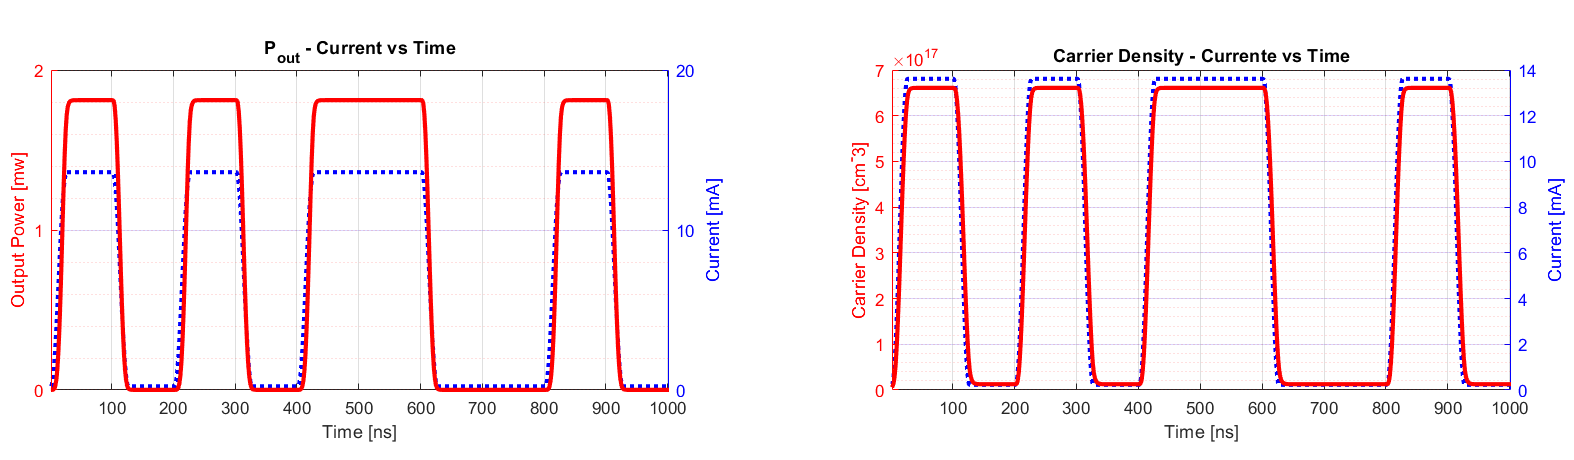
\includegraphics[width=13cm]{lab2/Images/prob3/10M.png}
  \caption{Risposta temporale a $10\text{ Mbit/s}$.}
  \label{fig:10M}
\end{figure}

\vspace{-0.25cm}

\begin{figure}[!h]
 \centering
 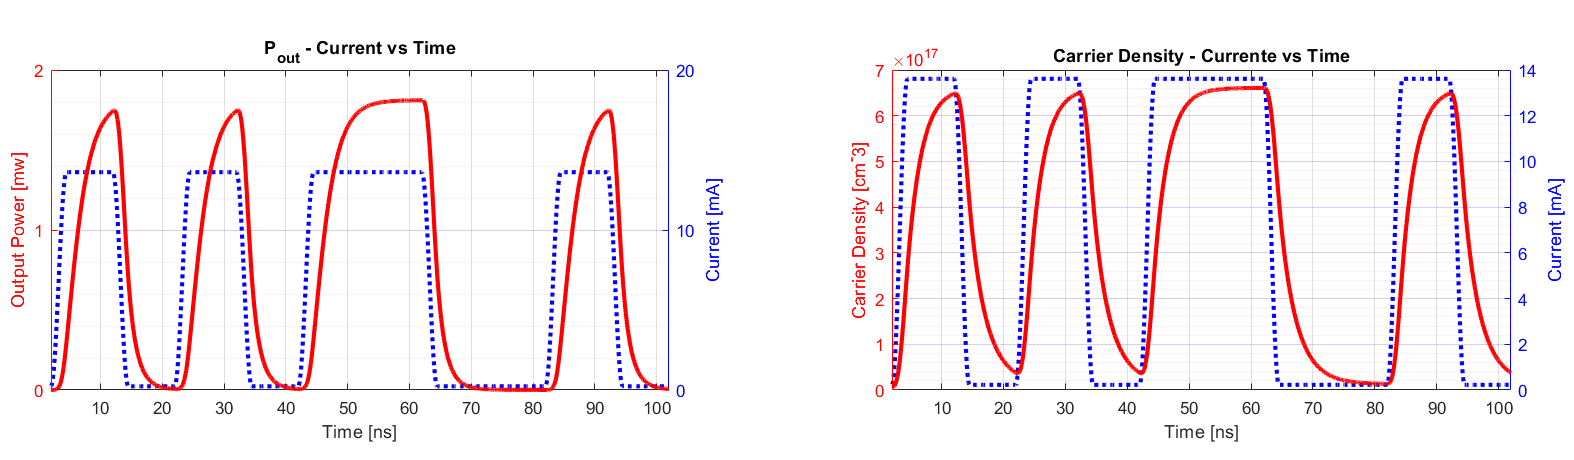
\includegraphics[width=13cm]{lab2/Images/prob3/100M.png}
  \caption{Risposta temporale a $100\text{ Mbit/s}$.}
  \label{fig:100M}
\end{figure}

\vspace{-0.25cm}

\begin{figure}[!h]
 \centering
 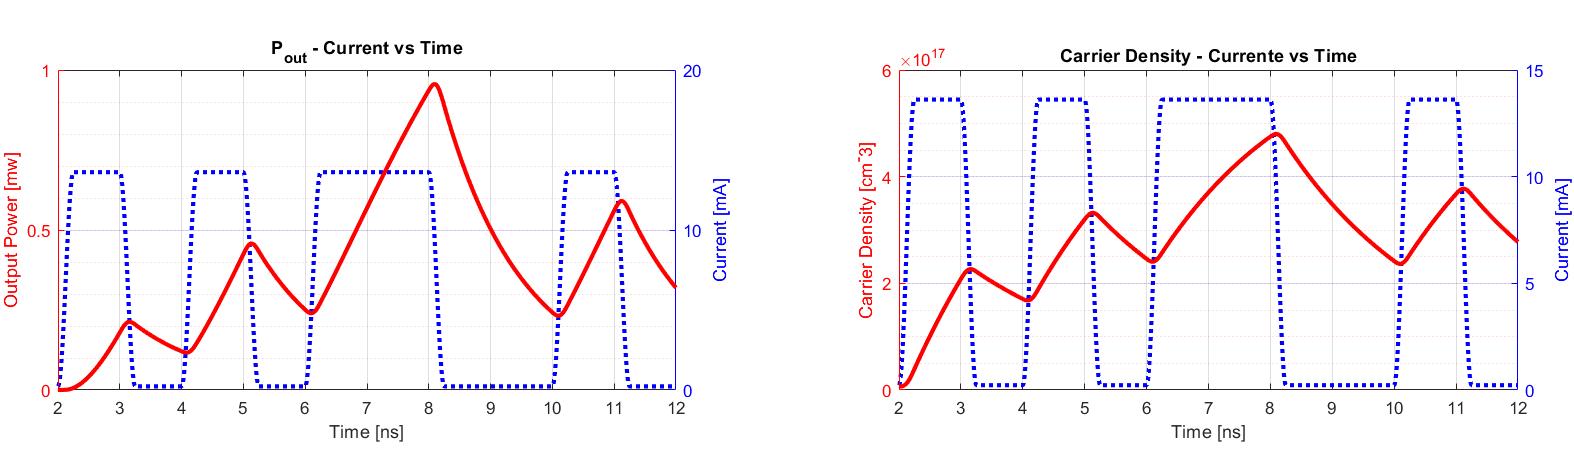
\includegraphics[width=13cm]{lab2/Images/prob3/1G.png}
  \caption{Risposta temporale a $1\text{ Gbit/s}$.}
  \label{fig:1G}
\end{figure}

\vspace{-0.25cm}

\begin{figure}[!h]
 \centering
 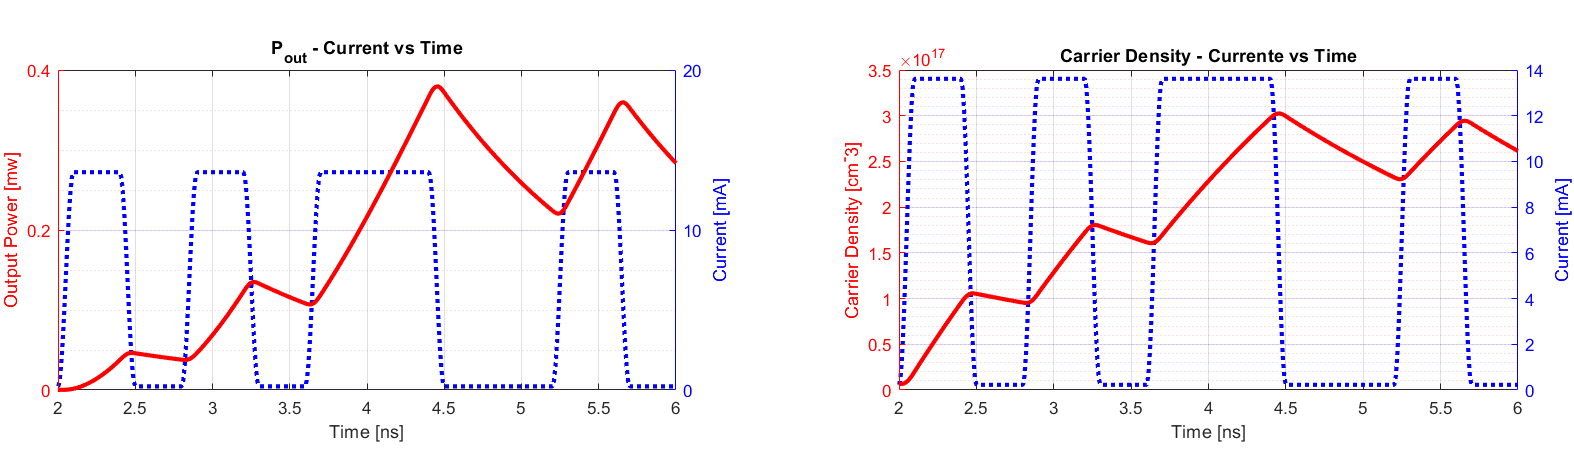
\includegraphics[width=13cm]{lab2/Images/prob3/2_5G.png}
  \caption{Risposta temporale a $2.5\text{ Gbit/s}$.}
  \label{fig:2_5G}
\end{figure}

\noindent\\ Dall'analisi dei transitori temporali si evidenziano tre regimi di funzionamento distinti:
\begin{itemize}
    \item \textbf{Basse frequenze ($10\text{ Mbit/s}$):} Il periodo di bit $T_b$ è sufficientemente lungo rispetto al tempo di vita dei portatori $\tau$.
    Il segnale ottico segue fedelmente la corrente di modulazione, raggiungendo perfettamente il valore di regime stazionario sia per i bit $1$ che per i bit $0$.
    \item \textbf{Medie frequenze ($100\text{ Mbit/s}$):} Il segnale segue ancora l'andamento della corrente, ma durante sequenze rapide e alternate di bit singoli
    ($0101\dots$) la densità di portatori non ha il tempo sufficiente per completare la carica o la scarica della regione attiva. Ciò porta a una parziale attenuazione
    dei livelli logici, anche se l'errore di trasmissione rimane molto basso.
    \item \textbf{Alte frequenze ($1\text{ Gbit/s}$ e $2.5\text{ Gbit/s}$):} La velocità di commutazione supera nettamente la frequenza di taglio del dispositivo
    ($f_{-3\text{dB}} \approx 100\text{ MHz}$). La potenza ottica non riesce più a seguire le variazioni della corrente, causando una severa distorsione del segnale e
    rendendo impossibile la distinzione dei livelli logici.
\end{itemize}

\noindent\\ Per convalidare quantitativamente queste osservazioni e valutare l'interferenza intersimbolica (ISI), sono stati estratti i \textbf{diagrammi ad occhio}
(\textit{eye diagrams}) a diversi valori del bit-rate ($10\text{ Mbit/s}$, $100\text{ Mbit/s}$, $200\text{ Mbit/s}$, $500\text{ Mbit/s}$, $1\text{ Gbit/s}$ e
$2.5\text{ Gbit/s}$), riportati nelle Figure seguenti.


\begin{figure}[!h]
 \centering
 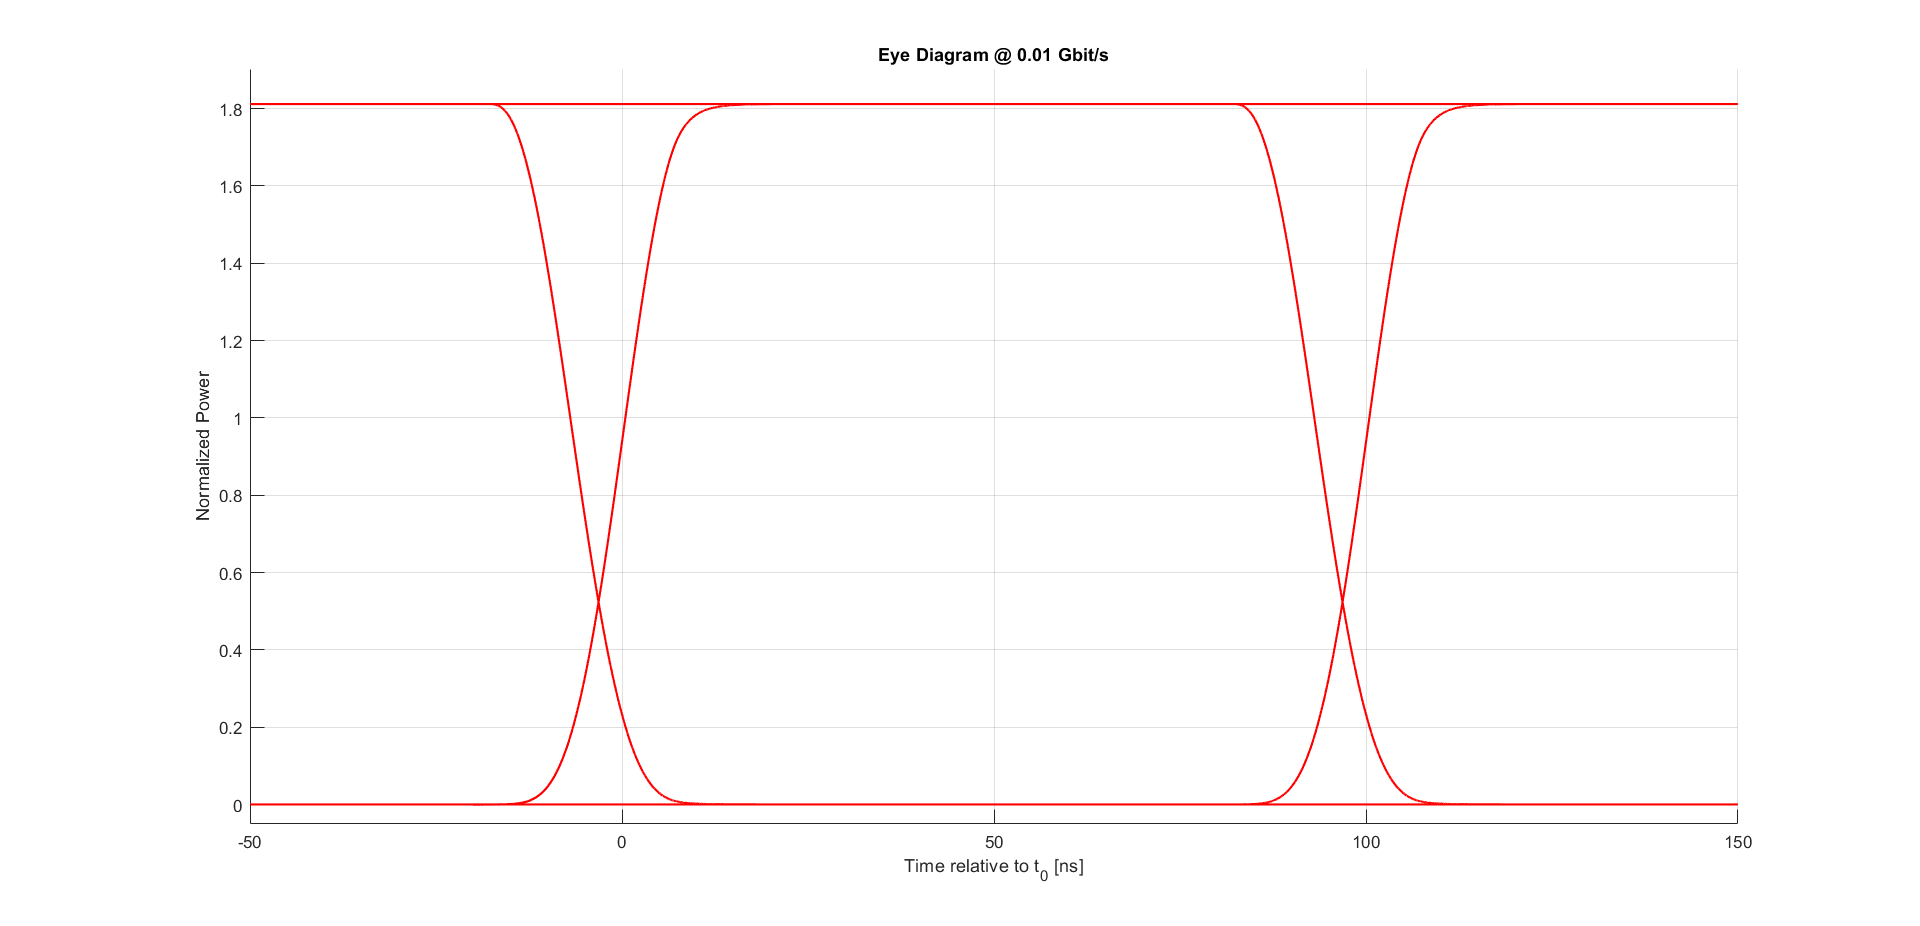
\includegraphics[width=14.5cm]{lab2/Images/prob3/eye_10M.png}
  \caption{Diagramma ad occhio con $B_r = 10\text{ Mbit/s}$}
  \label{fig:eye_10M}
\end{figure}

\begin{figure}[!h]
 \centering
 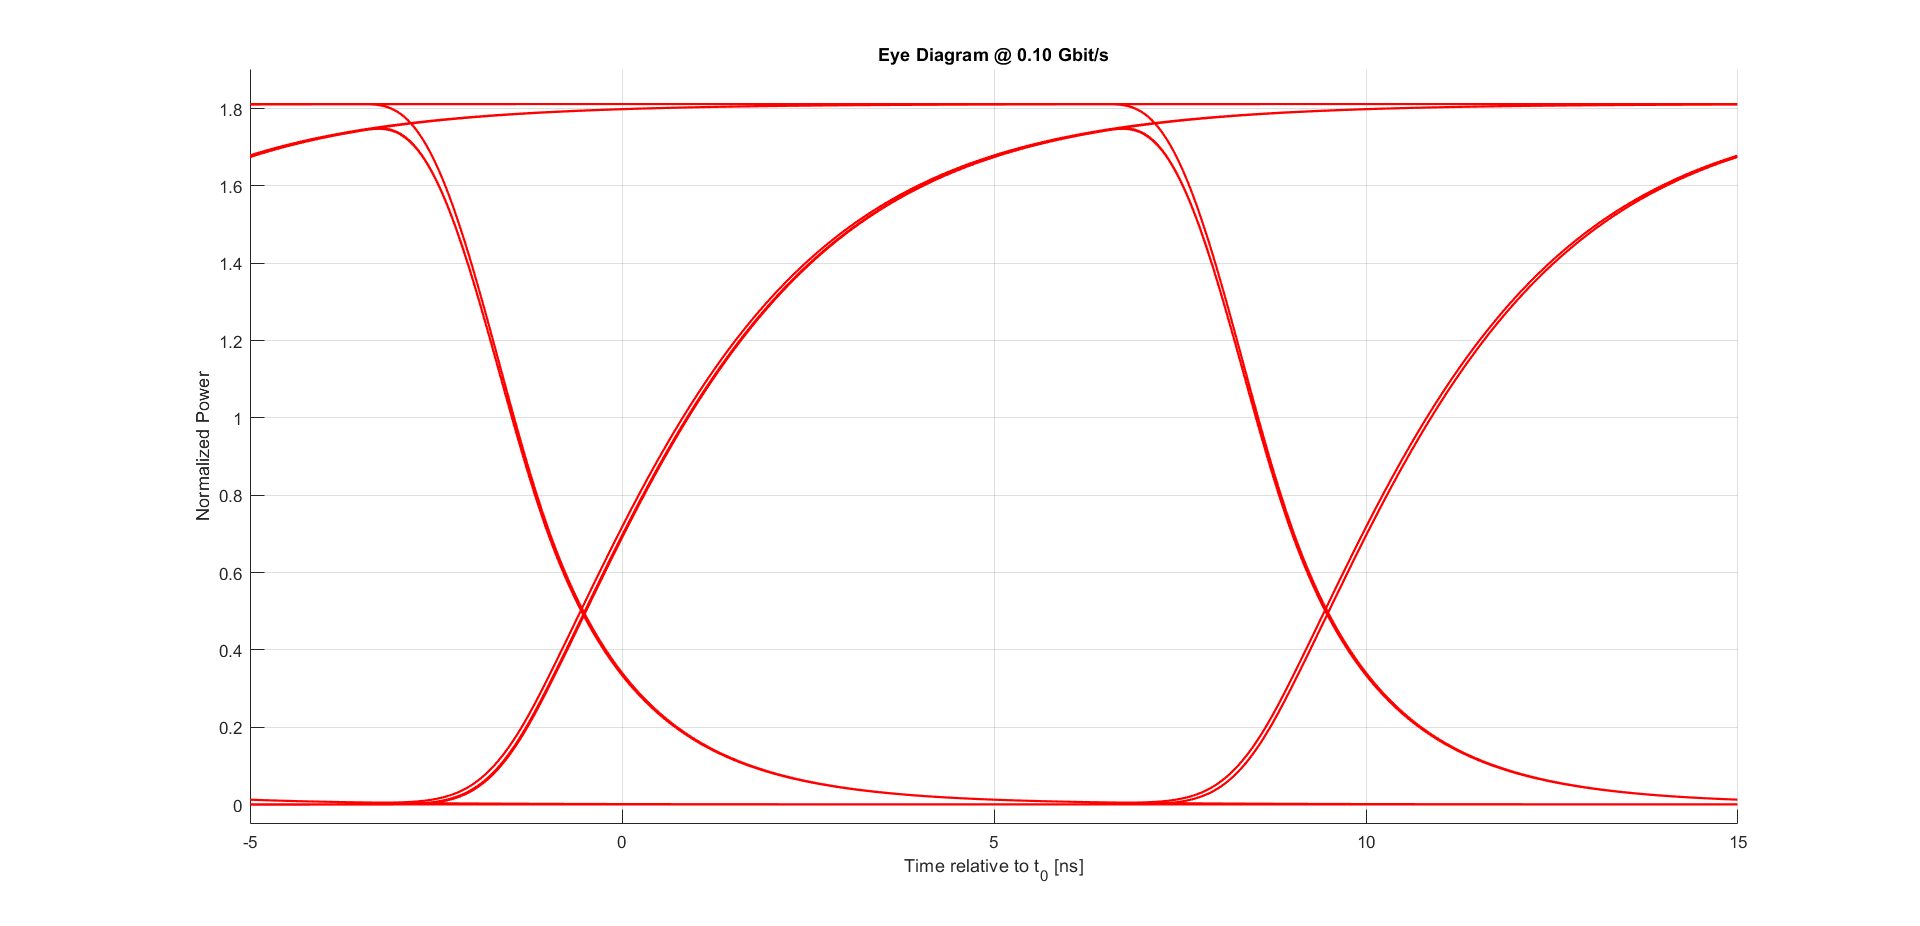
\includegraphics[width=14.5cm]{lab2/Images/prob3/eye_100M.png}
  \caption{Diagramma ad occhio con $B_r = 100\text{ Mbit/s}$}
  \label{fig:eye_100M}
\end{figure}

\begin{figure}[!h]
 \centering
 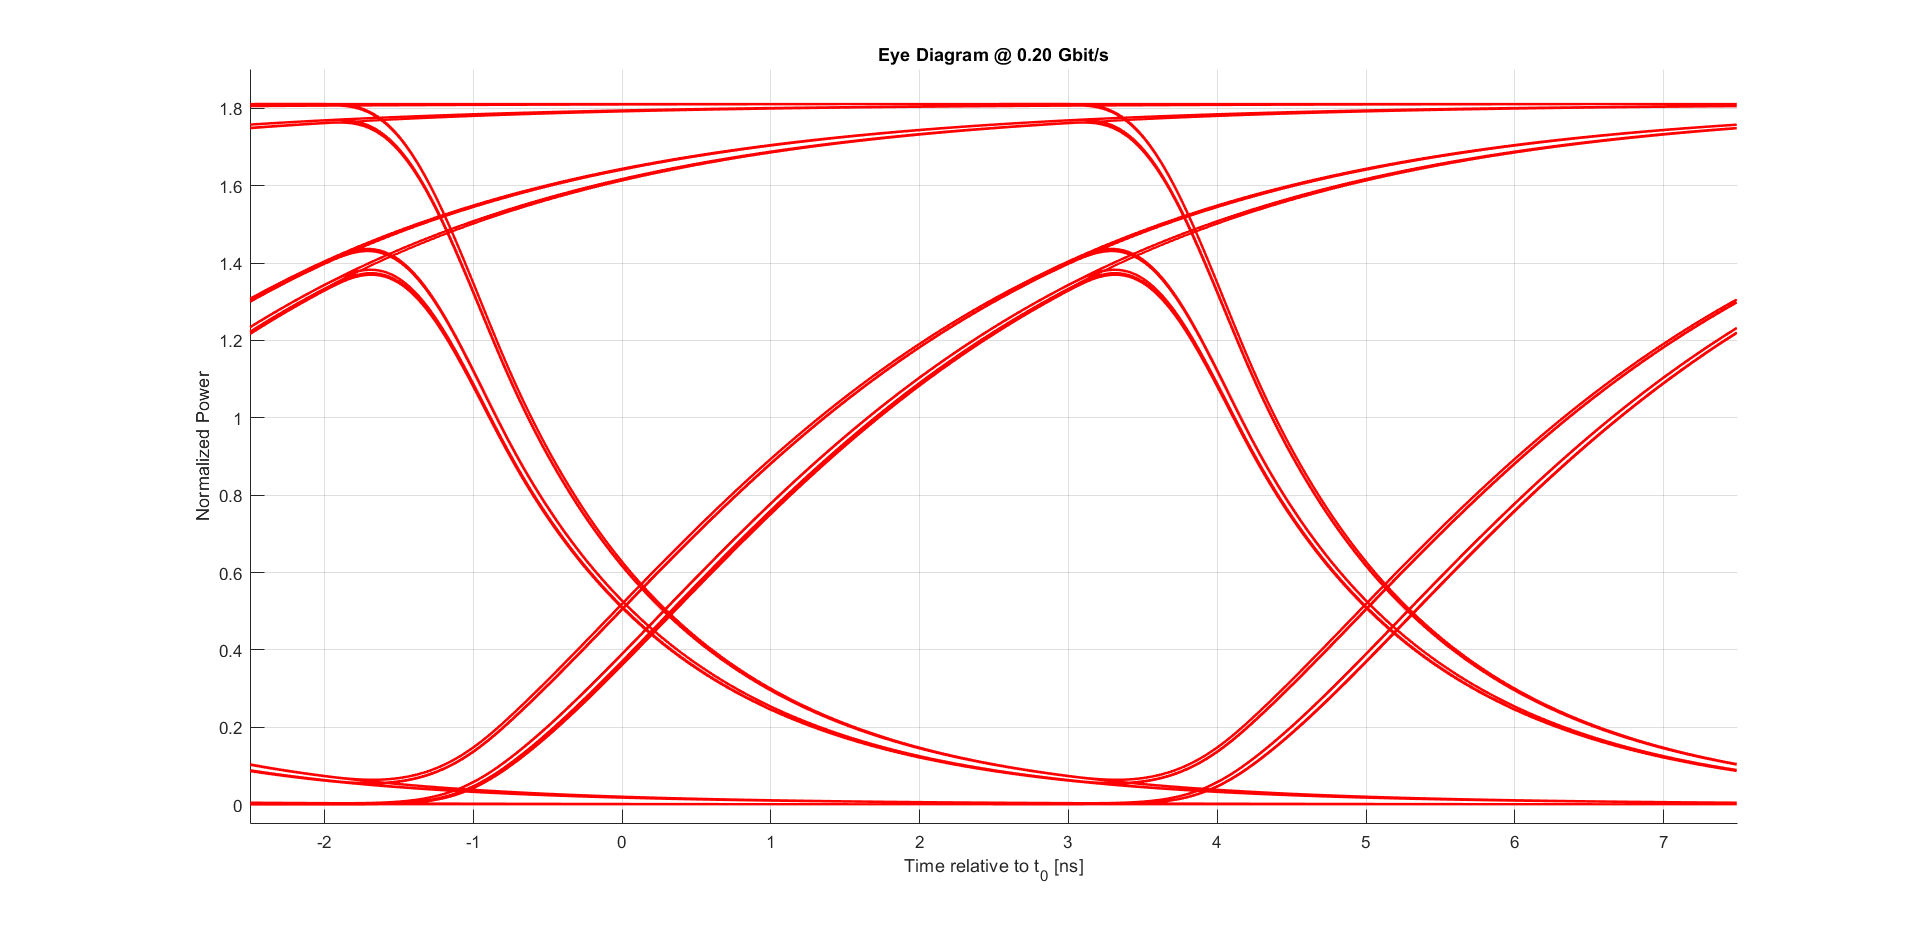
\includegraphics[width=14.5cm]{lab2/Images/prob3/eye_200M.png}
  \caption{Diagramma ad occhio con $B_r = 200\text{ Mbit/s}$}
  \label{fig:eye_200M}
\end{figure}

\begin{figure}[!h]
 \centering
 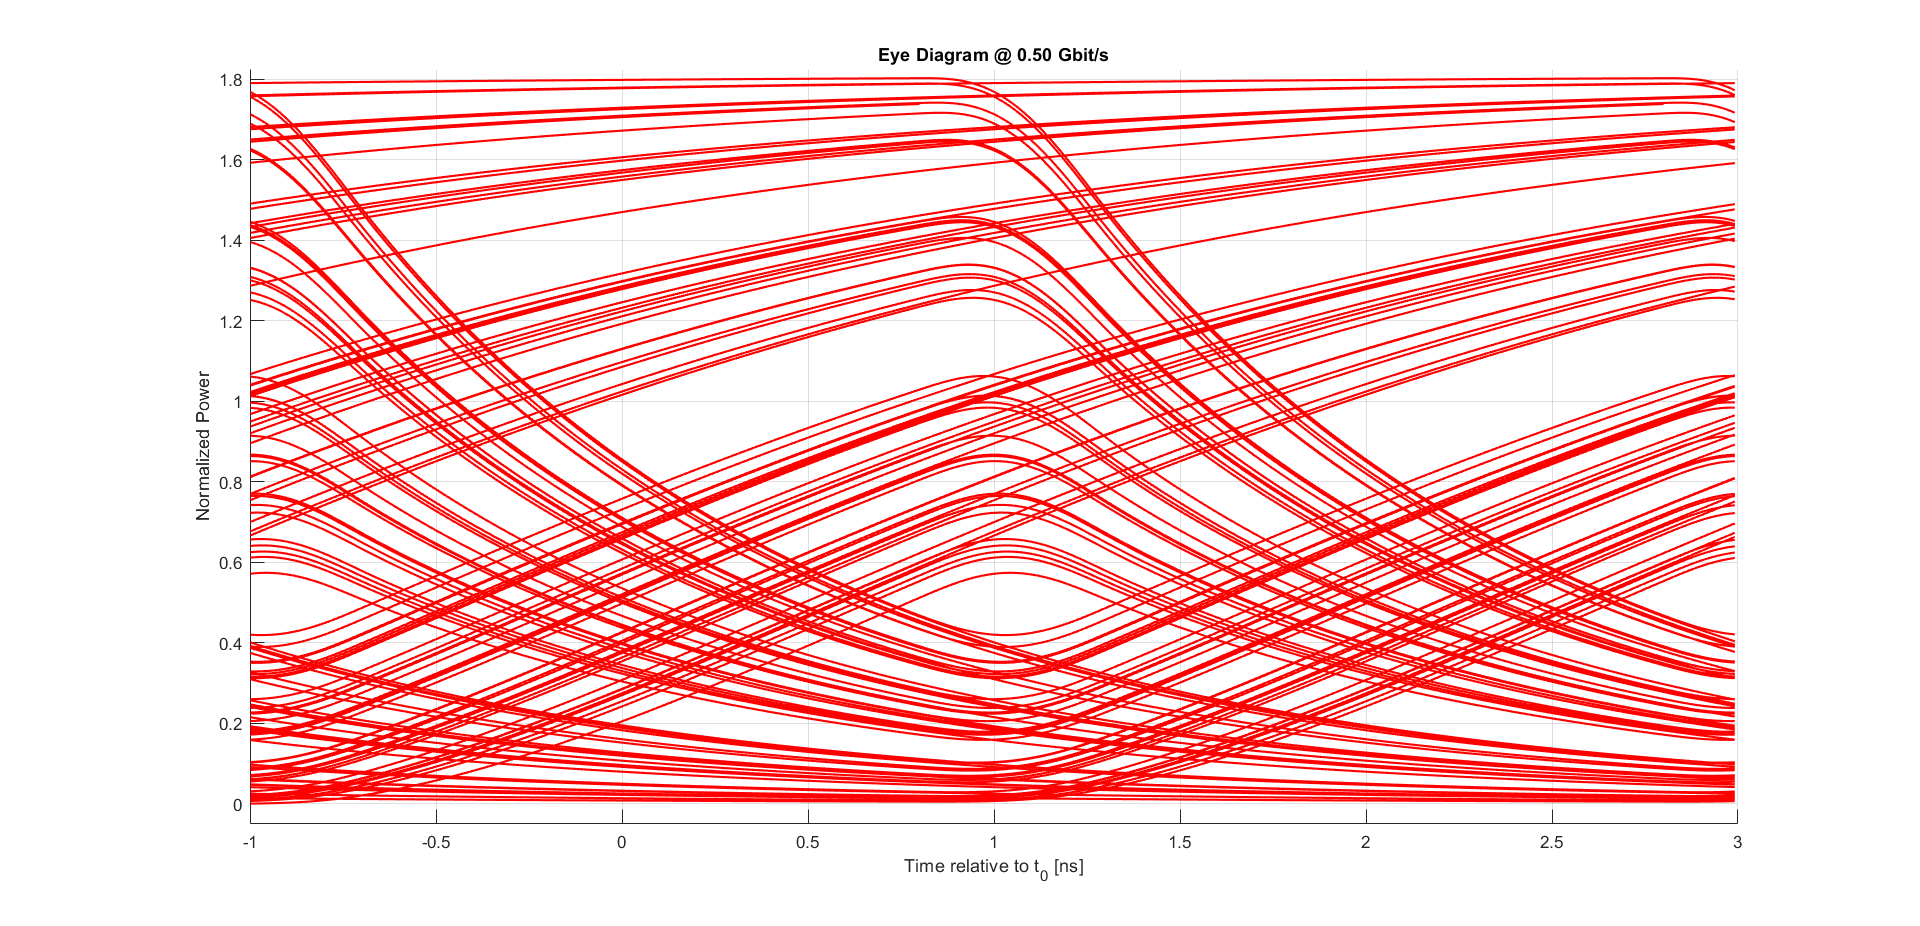
\includegraphics[width=14.5cm]{lab2/Images/prob3/eye_500M.png}
  \caption{Diagramma ad occhio con $B_r = 500\text{ Mbit/s}$}
  \label{fig:eye_500M}
\end{figure}

\begin{figure}[!h]
    \centering
    \begin{subfigure}[b]{0.48\textwidth}
        \centering
        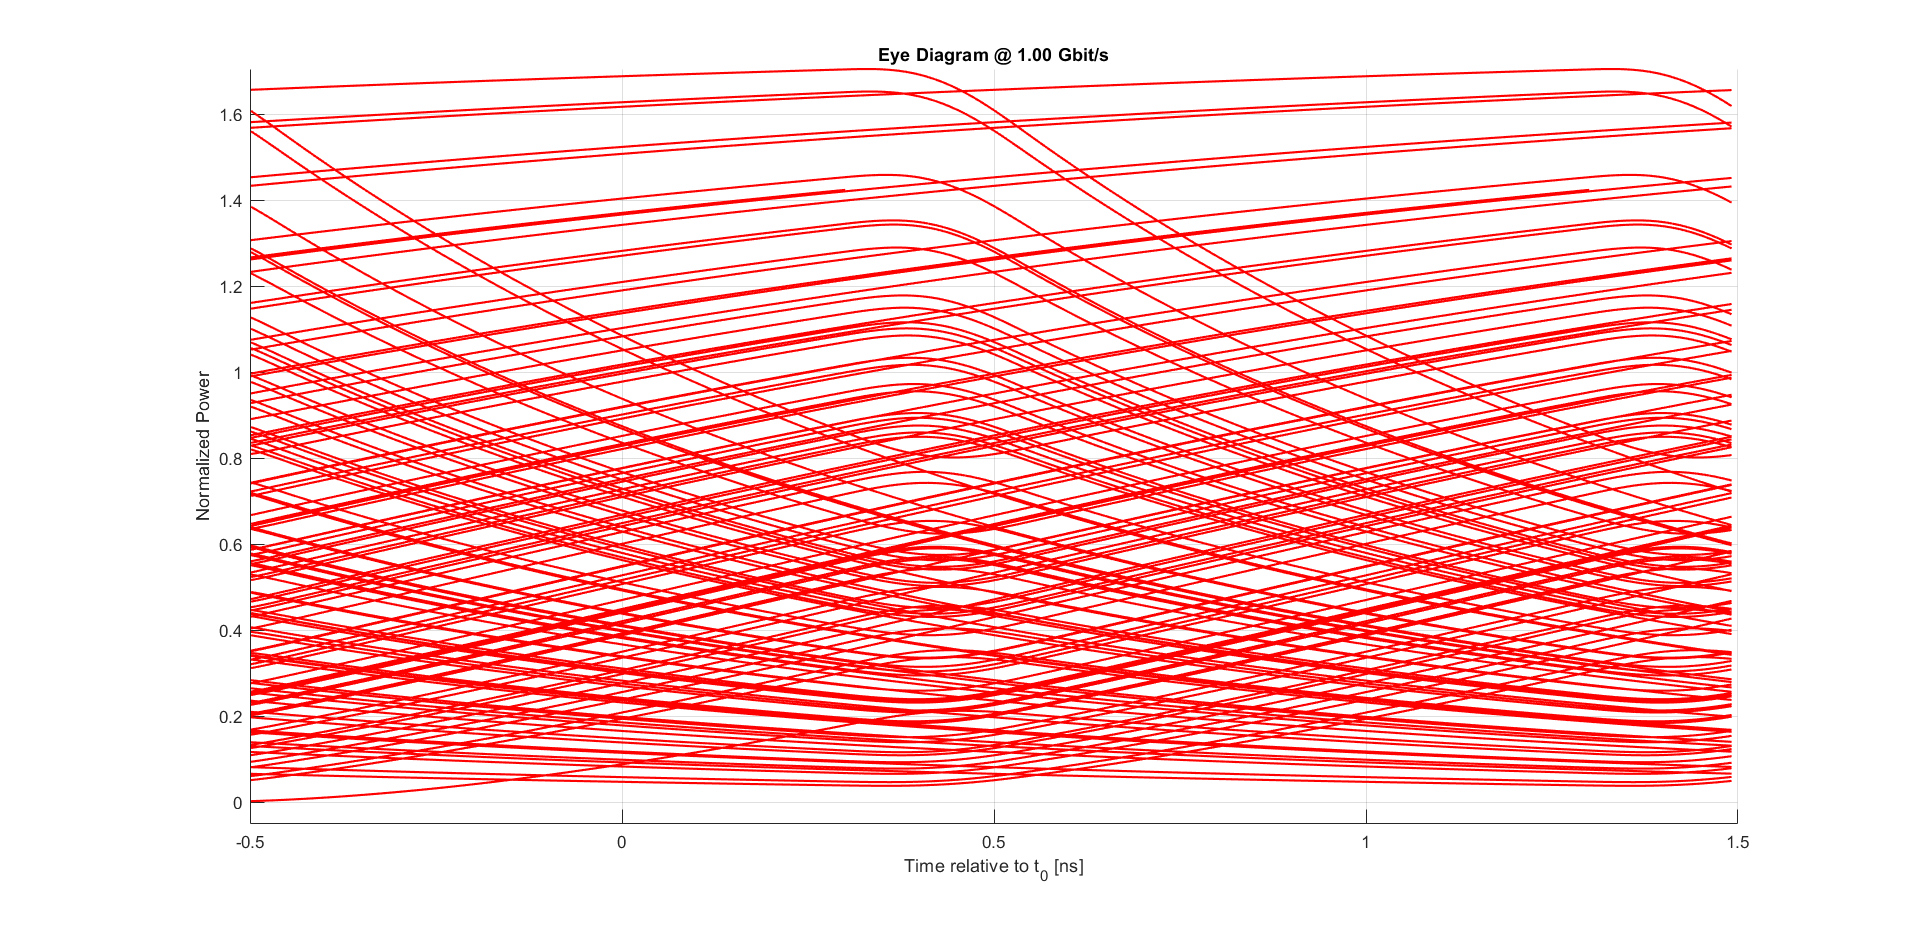
\includegraphics[width=\textwidth]{lab2/Images/prob3/eye_1G.png}
        \caption{Diagramma ad occhio con $B_r = 1\text{ Gbit/s}$}
        \label{fig:eye_1G}
    \end{subfigure}
    \hfill
    \begin{subfigure}[b]{0.48\textwidth}
        \centering
        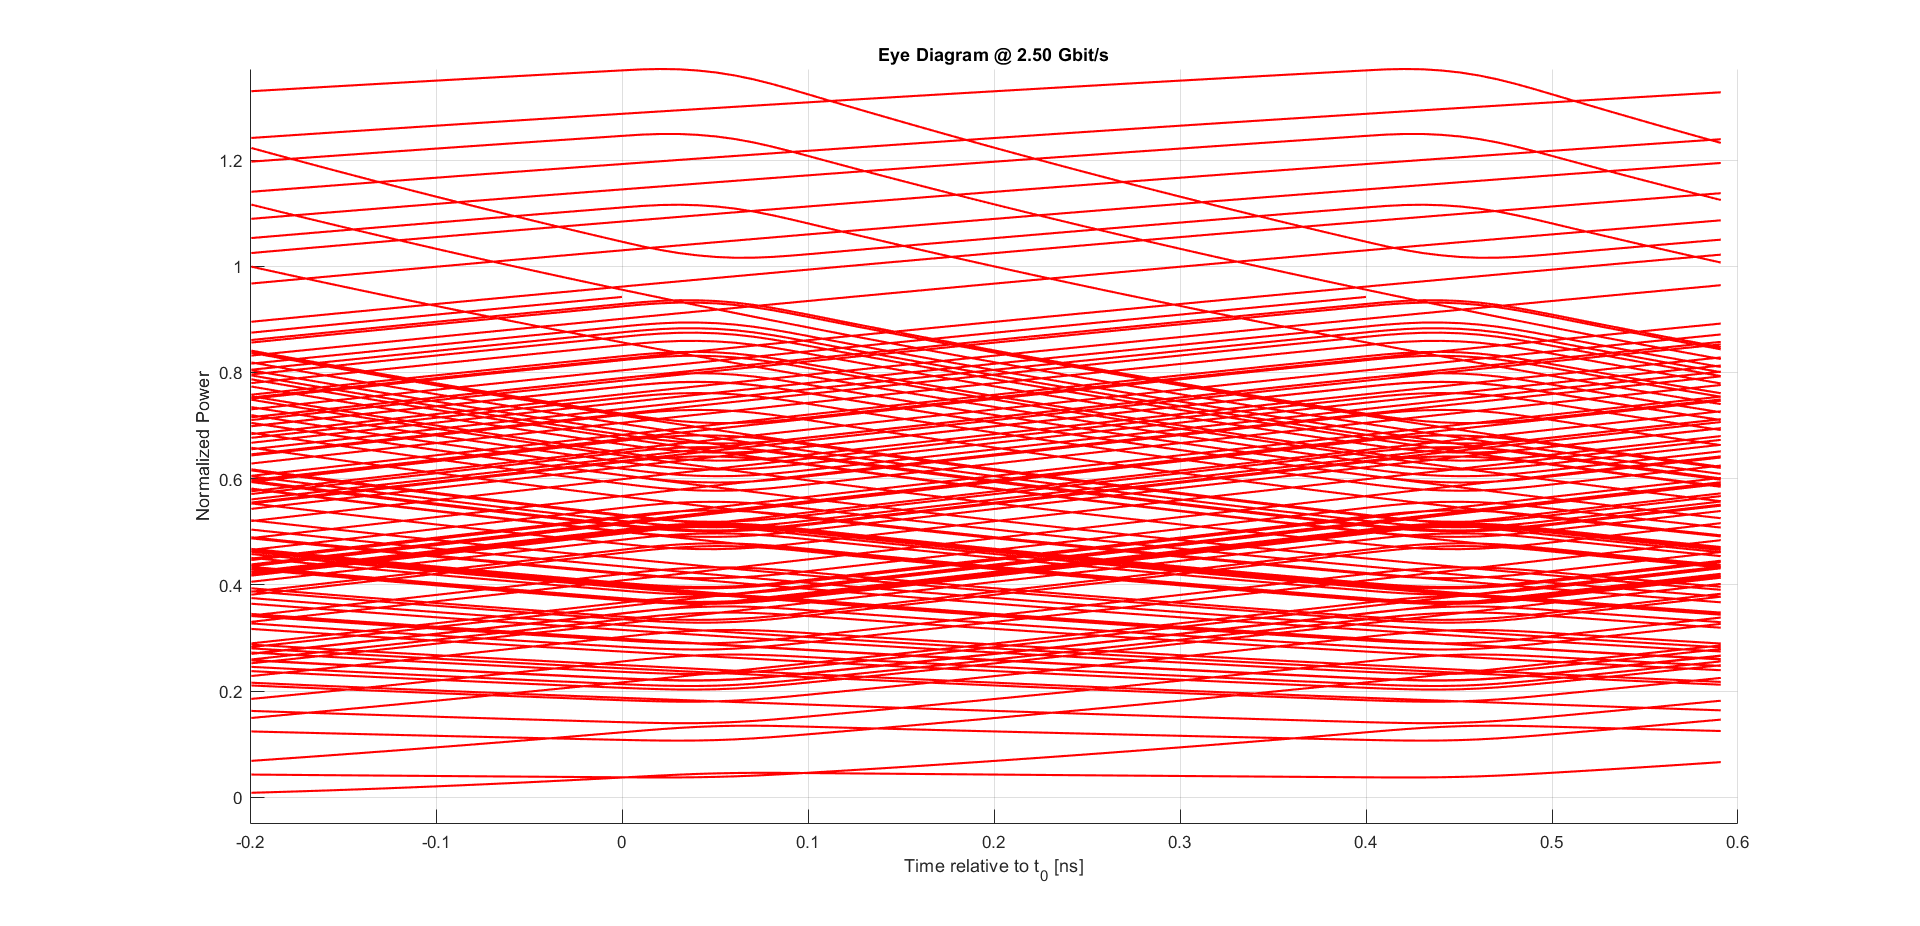
\includegraphics[width=\textwidth]{lab2/Images/prob3/eye_2.5G.png}
        \caption{Diagramma ad occhio con $B_r = 2.5\text{ Gbit/s}$}
        \label{fig:eye_2.5G}
    \end{subfigure}
    \caption{Diagrammi ad occhio a bit-rate molto elevati}
    \label{fig:eye_Gbs}
\end{figure}

\noindent L'analisi dei diagrammi ad occhio conferma direttamente il degrado delle prestazioni:
\begin{itemize}
    \item A \textbf{10 Mbit/s}, l'occhio è ben definito e mostra un'ampia apertura, indicando un'ottima immunità al rumore. Si ha un ottimo margine di separazione tra i livelli logici e una limitata interferenza intersimbolica.
    \item A \textbf{100 Mbit/s}, l'occhio mantiene un'ottima apertura verticale e orizzontale, consentendo di conciliare le prestazioni con un margine di rumore sicuro.
    \item A \textbf{200 Mbit/s}, il diagramma inizia a mostrare i primi effetti evidenti dell'interferenza intersimbolica (ISI). L'apertura dell'occhio rimane comunque
    sufficiente a garantire una trasmissione corretta, ma si nota una riduzione dell'apertura verticale dovuta alla lentezza della dinamica di carica della regione attiva
    (fronti di salita più lenti rispetto a quelli di discesa).
    \item A \textbf{500 Mbit/s}, il diagramma mostra una chiusura pressoché totale dell'occhio, sia in senso verticale che orizzontale. Poiché il bit-rate
    supera ampiamente la banda a $-3\text{ dB}$ del LED, l'effetto dell'interferenza intersimbolica (ISI) diventa dominante: la potenza ottica non riesce a raggiungere
    i livelli logici di regime prima della commutazione successiva, rendendo impossibile la scelta di un livello di soglia per il campionamento e portando inevitabilmente a 
    degli errori di trasmissione.
    \item A frequenze maggiori, ovvero a \textbf{1 Gbit/s} e \textbf{2.5 Gbit/s}, il diagramma ad occhio risulta completamente chiuso e distorto; l'elevata interferenza
    intersimbolica rende il segnale del tutto indecodificabile e la trasmissione inadatta a qualsiasi applicazione di comunicazione.
\end{itemize}